\documentclass[slidestop,compress,mathserif]{beamer} 
% 
\mode<presentation> 
% 
% 
\usetheme{Antibes}
\usepackage{verbatim}
\usepackage{lmodern} 
%\usepackage[german]{babel} 
\usepackage[english]{babel}
\usepackage{amsmath} 
\usepackage{mathrsfs} 
\usepackage{dsfont} 
\usepackage{ulem}
\usepackage{tikz}
\usepackage{multicol}
\usepackage{enumerate}
\usepackage{marvosym}
\usepackage{capt-of}
\usepackage{lipsum}

\usetikzlibrary{arrows.meta,shapes.arrows}
 
%\usepackage{float} 
%%%%%%%%%%%%Essential Supremum and Infimum definitions%%%%%%%%%%%%%
\DeclareMathOperator*{\esssup}{ess\sup} 
\DeclareMathOperator*{\essinf}{ess\inf} 
%%%%%%%%%%%%end definitions%%%%%%%%%%%%%%%%%%%%%%%%%% 
\setbeamercolor*{block title example}{bg=red} 
\setbeamercolor*{block body example}{fg= black, bg= red} 
\usepackage{xcolor} 
%%%%%%%%%%%% Color definitions %%%%%%%%%%%%%%%%%% 
\def\black#1{\textcolor{black}{#1}} 
\def\blue#1{\textcolor{blue}{#1}} 
\def\red#1{\textcolor{red}{#1}} 
\def\green#1{\textcolor{green}{#1}} 
\def\yellow#1{\textcolor{yellow}{#1}} 
%%%%%%%%%%%%%%% end definitions %%%%%%%%%%%%%%%%%%%%%%%% 
\usepackage{beamerthemeshadow} 
% 
\setbeamercolor*{leftfootline}{fg=white,bg=blue} 
\setbeamercolor*{rightfootline}{fg=blue,bg=white} 
% 
\setbeamertemplate{footline}{% 
\leavevmode% 
\begin{beamercolorbox}[ht=2.5ex,dp=1.5ex,wd=0.3\paperwidth,center]{leftfootline} 
\insertauthor 
\end{beamercolorbox}% 
\begin{beamercolorbox}[ht=2.5ex,dp=1.5ex,wd=0.7\paperwidth,center]{rightfootline} 
\inserttitle 
\end{beamercolorbox} 
} 
% 
% 
\title{Systematic Studies for the $\pi^0$ Calibration of the Crystal-Ball Detector}   
\author{Martin Sobotzik} 
\institute{Johannes Gutenberg-Universit\"at Mainz} 
\date{xx.yy.2017} 
% 
\begin{document} 

\begin{frame} 
\titlepage 
\end{frame} 


\begin{frame} 
\frametitle{Table of Contents} 
\tableofcontents[currentsection]
\end{frame} 
\section{Motivation}
\begin{frame}

		\frametitle{The Process}
	
		\begin{equation}
			\gamma + p \rightarrow \pi^0 +p \rightarrow p + \gamma_1 \gamma_2
		\end{equation}
		\begin{equation}
		m_{\pi^0}=\sqrt{2 E_1E_2(1-\text{cos}(\alpha))}
		\end{equation}
		\pause
			\begin{itemize}
		\item How can it be checked if there is a energy dependency in the CB?
		\pause
		 
		 
		 $\rightarrow |E_1 - E_2|<25\,\text{MeV}$
		\pause

		\item What are the reasons for the dependency?
	\end{itemize}
\end{frame}

\section{Preparation}
\begin{frame}
	\frametitle{Crystal-Ball-Function / Reduction of the Underground}
	\begin{itemize}
		\item Gaussian Fit Function $\rightarrow$ Crystal-Ball Fit Function
		\pause
		\item Check if the registered particles are charged 
		
		$\rightarrow$ Reduction of the underground
	\end{itemize}

\pause
\begin{figure}
	
		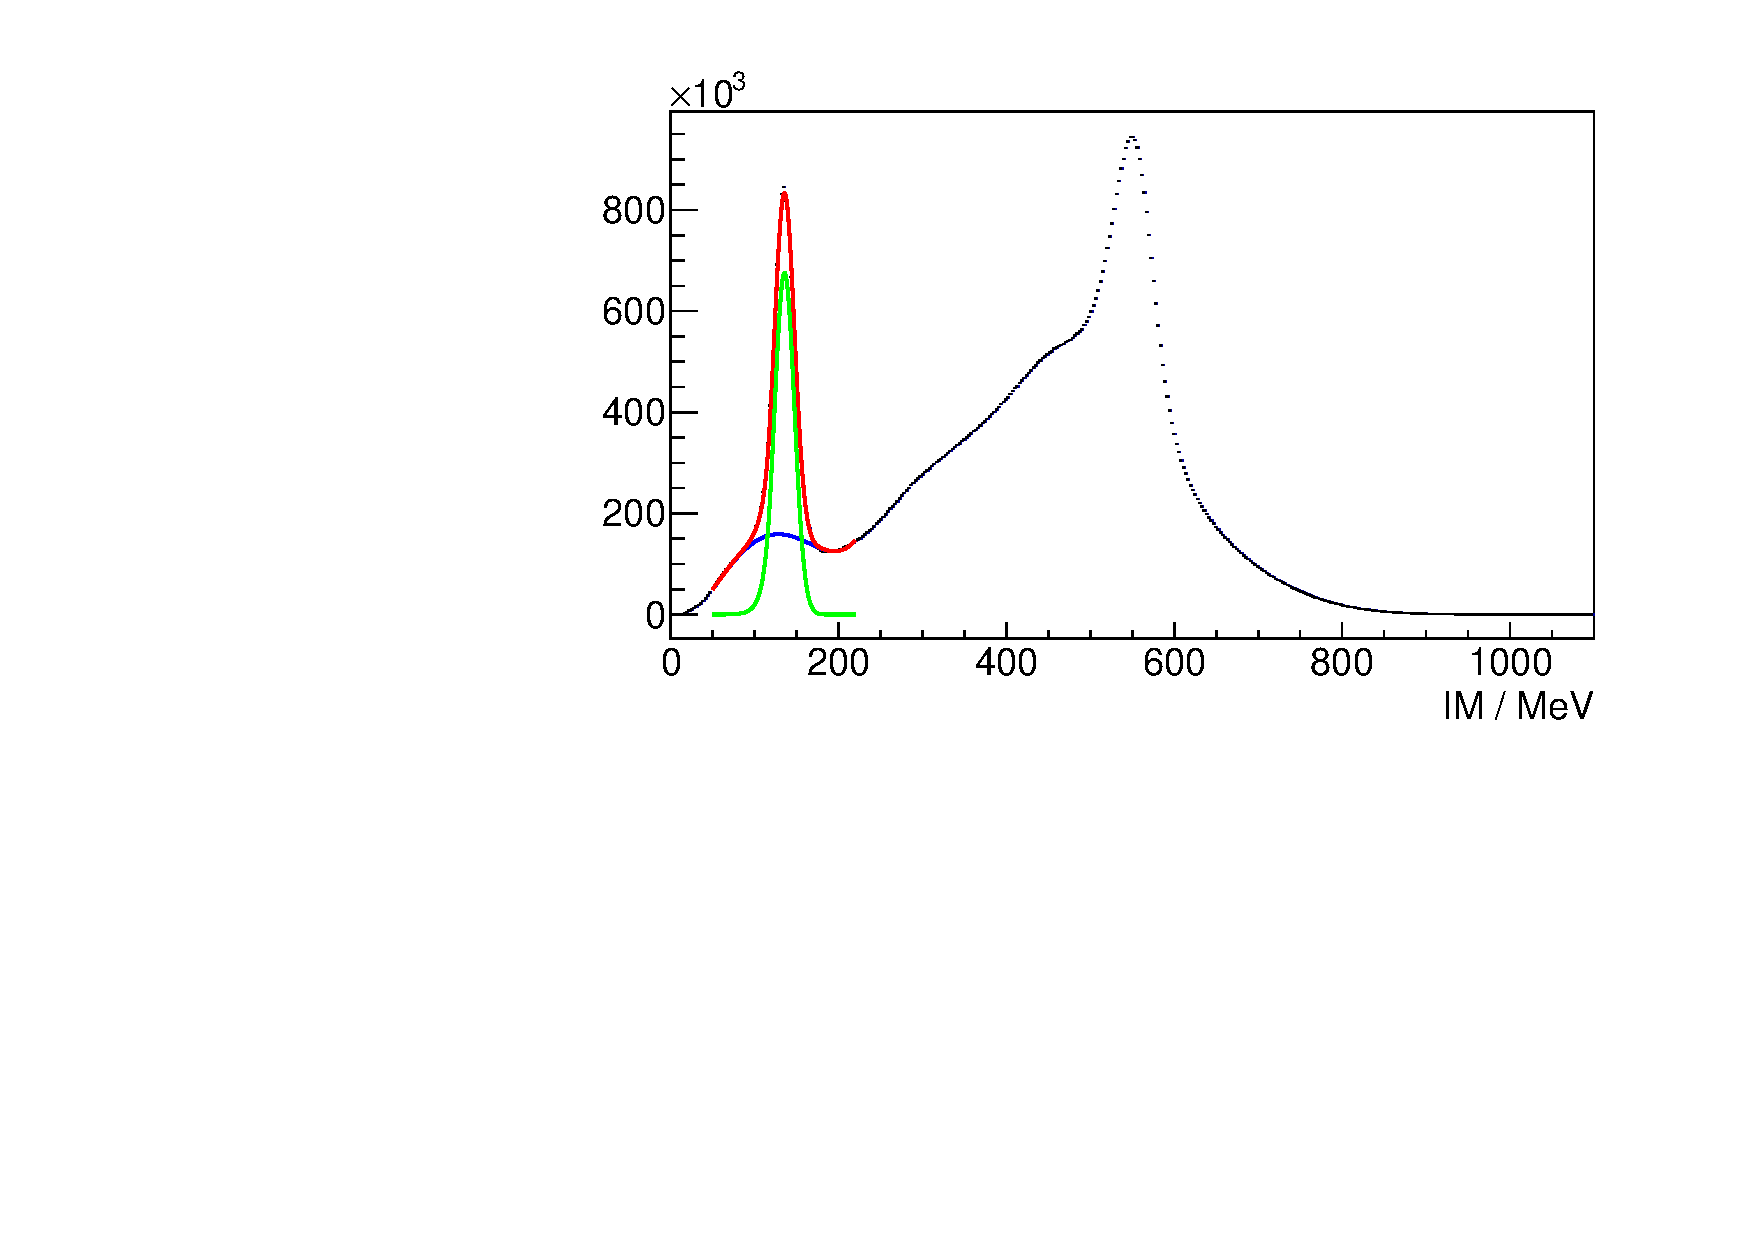
\includegraphics[width=0.50\textwidth]{Pictures/20171904RealIntervalFitExample}
	\hfill
		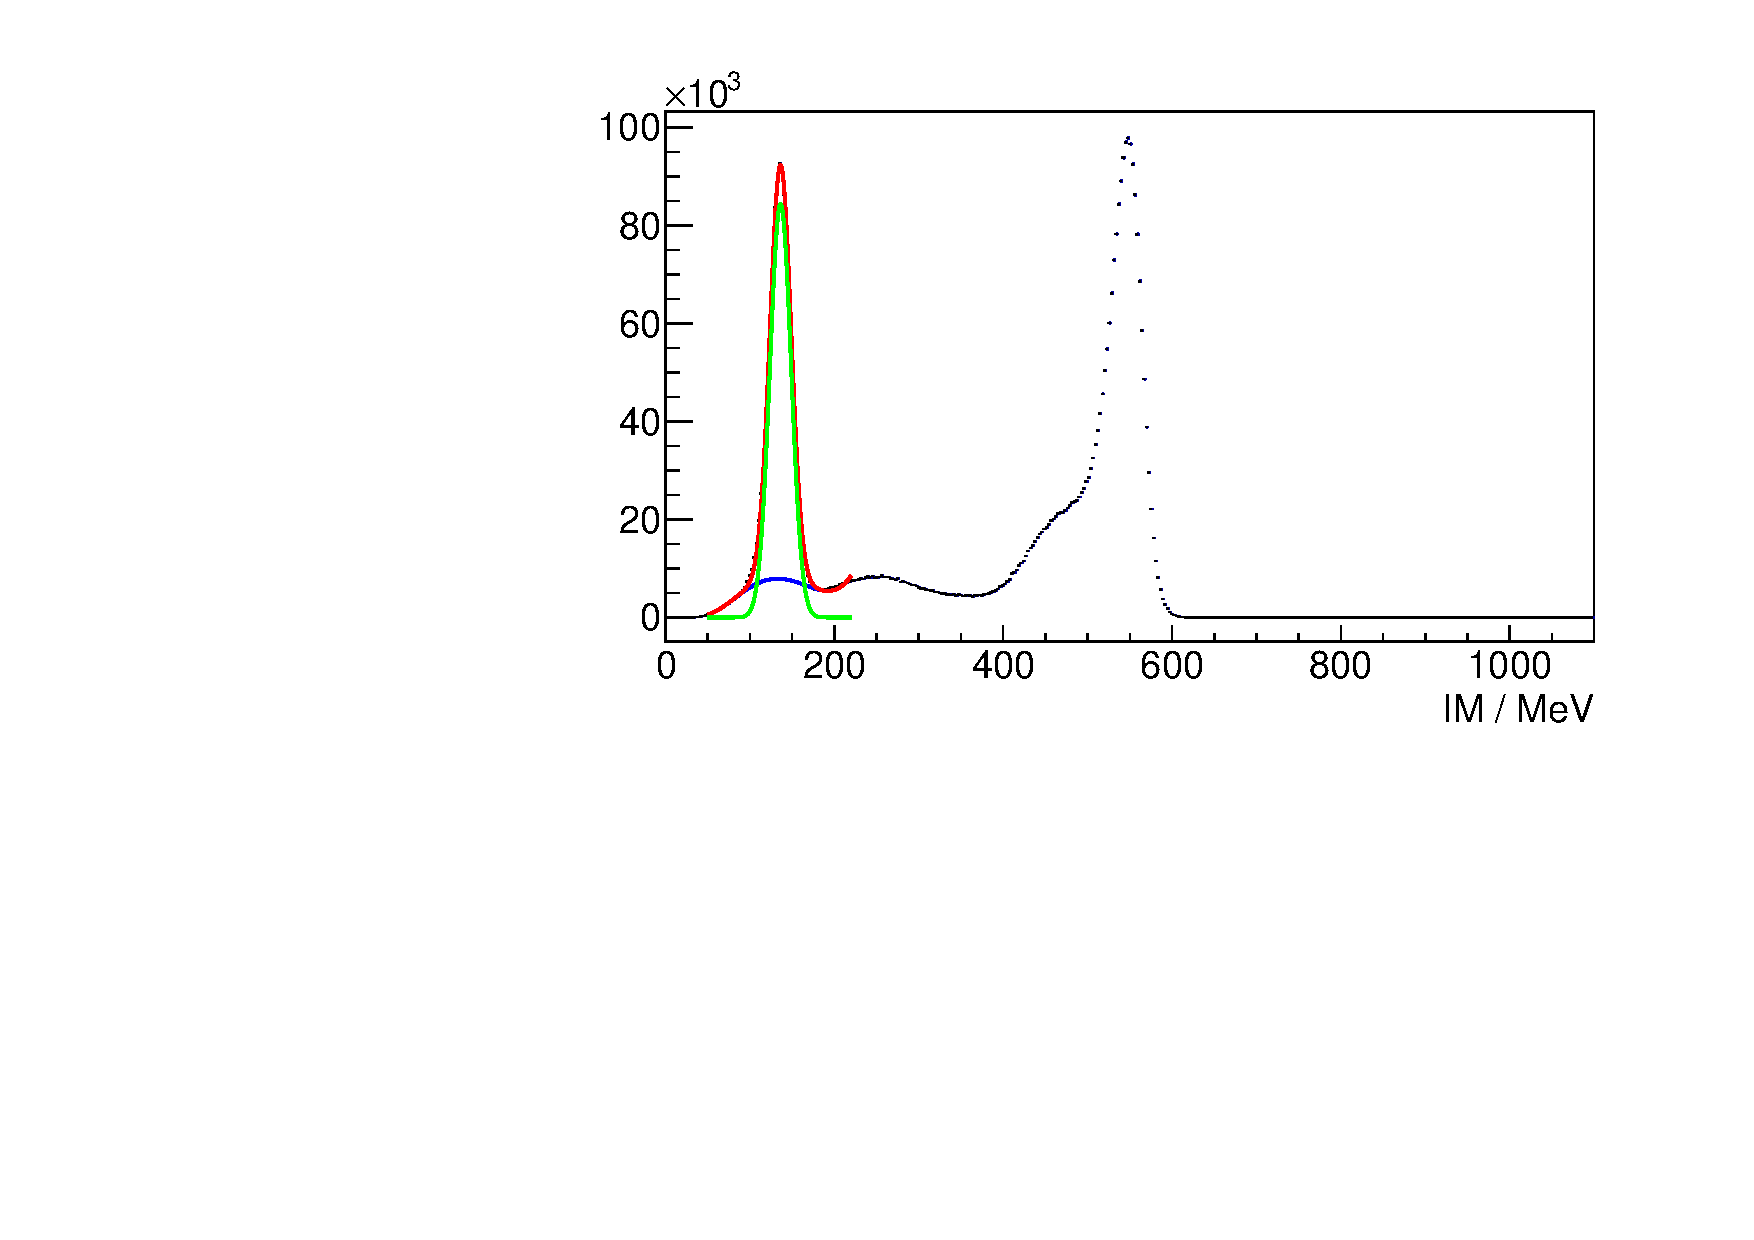
\includegraphics[width=0.50\textwidth]{Pictures/20171904RealUnchargedFitExample}
		\caption{Beamtime: Example for not reduced and reduced underground}
\end{figure}
\begin{tikzpicture}[remember picture,overlay]   
\coordinate (b) at (5.0 , 3.5);
\coordinate (c) at (5.7 , 3.5);
\draw [thick,black, ->,thick] (b) -- (c);
\end{tikzpicture}

\end{frame}
\begin{frame}
\frametitle{Event Generator}
Reasons for a new event generator:
\pause
\begin{itemize}
	\item The condition $|E_1 - E_2|<25\,\text{MeV}$ is a strong cut 
	
	$\rightarrow$ There is no package with enough events
	\pause
	
	\item Creating a new package with enough events would take to much time (multiple days on blaster)
	\pause
	
	\item It would be better if the same generator is used for all studies
	
	$\rightarrow$ The generator should be able to simulate MAMI-Beam and isotropic decay 
\end{itemize}
\end{frame}

\begin{frame}
	\frametitle{Event Generator}
\end{frame}
\section{Studies}


\begin{frame}
	\frametitle{No Additional Cut }
	
	\begin{itemize}
		\item Beamtime October 2014
		\item No additional cut
\end{itemize}
	
		\begin{figure}
		
		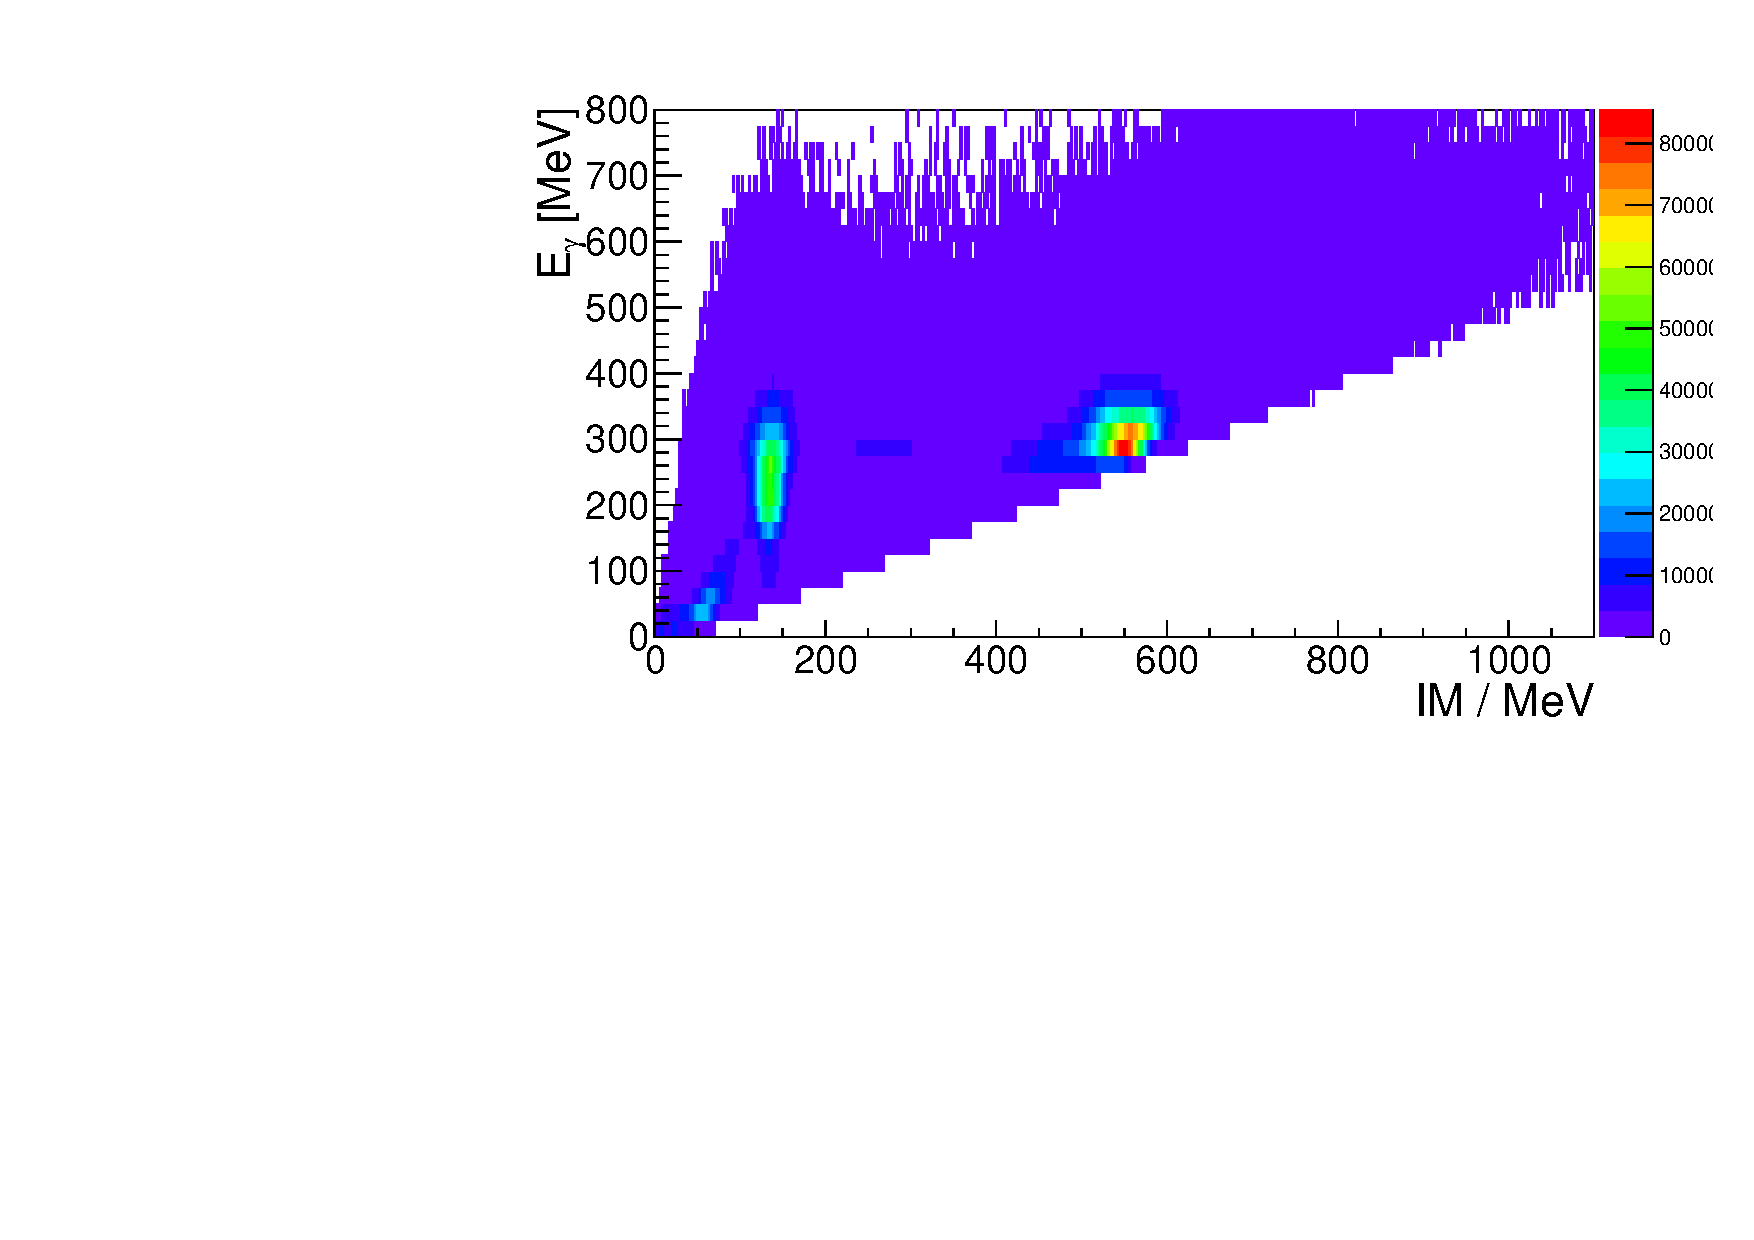
\includegraphics[width=0.50\textwidth]{Pictures/20171904Uncharged2DHist}
		\hfill
		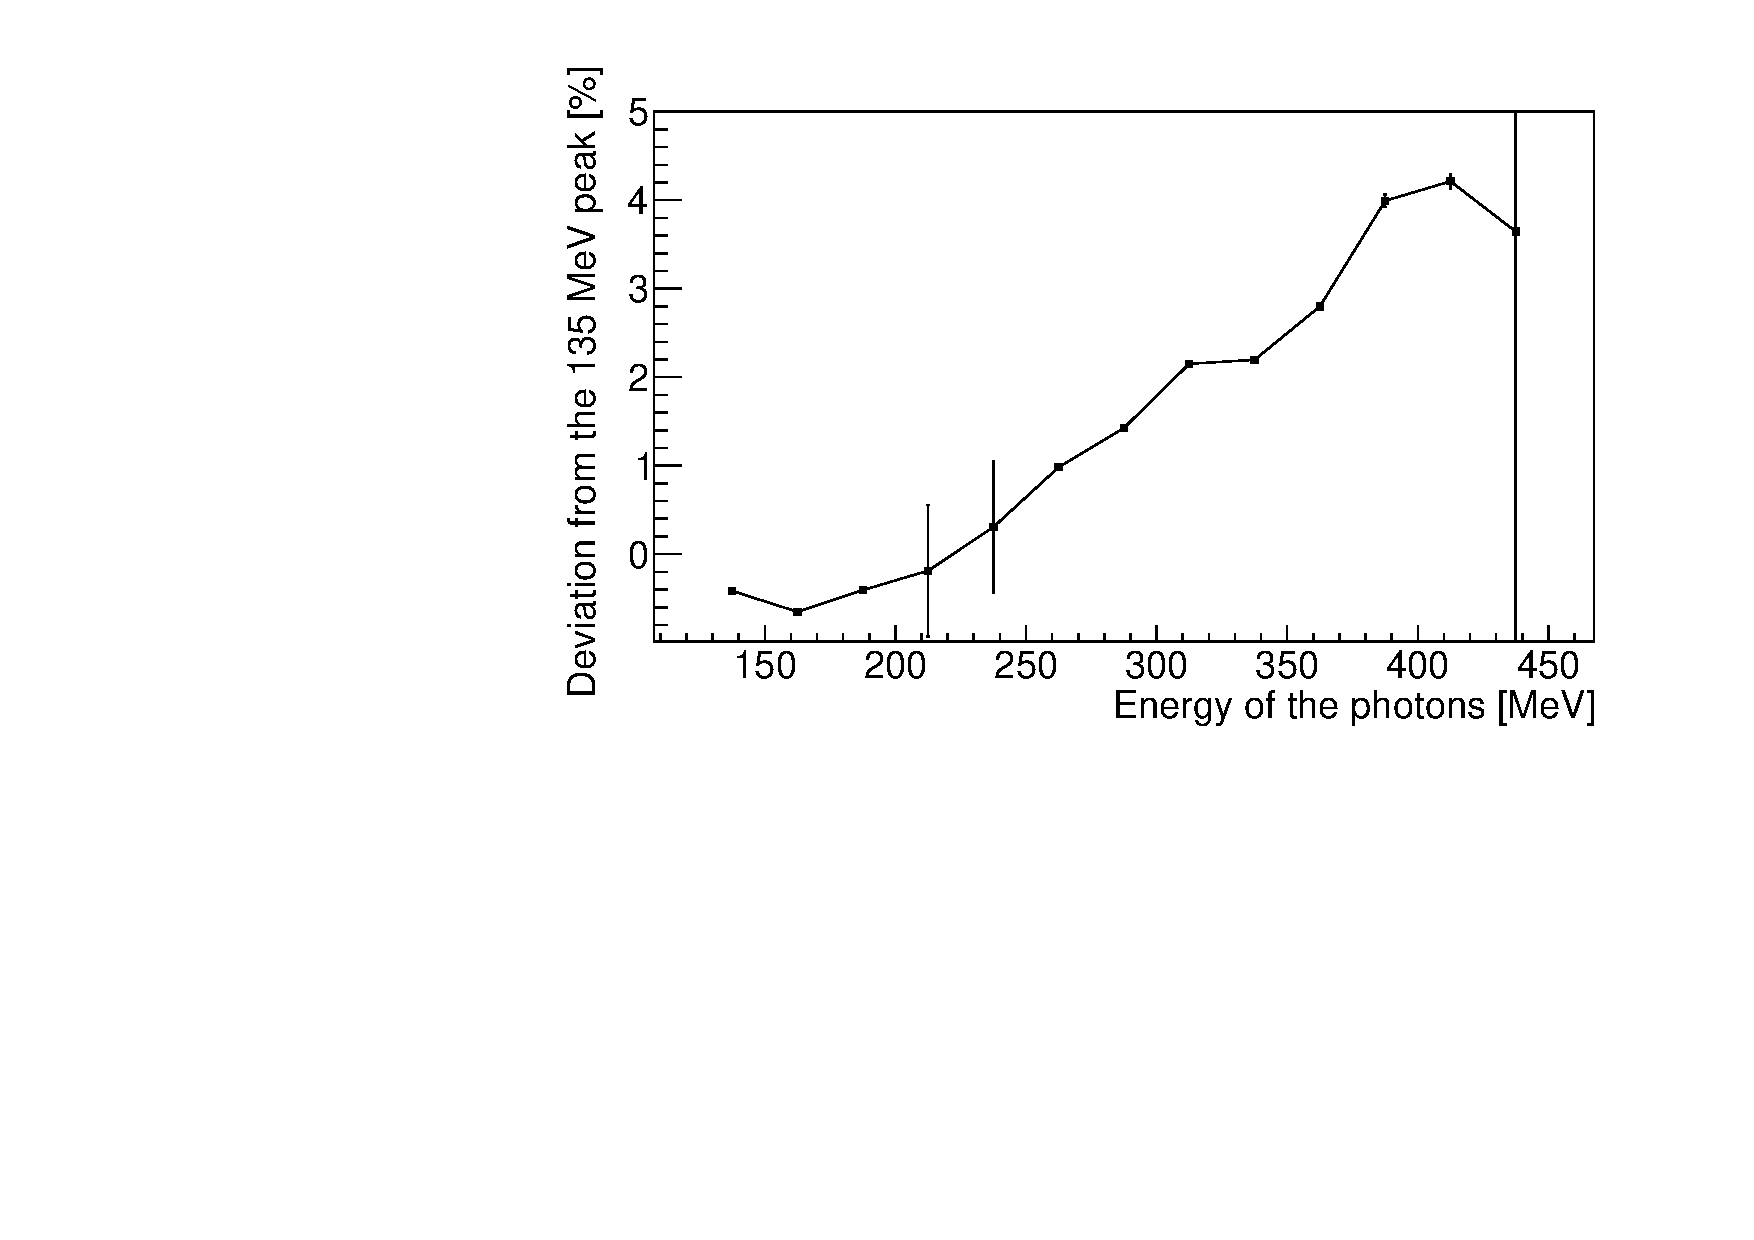
\includegraphics[width=0.50\textwidth]{Pictures/20170405StrahlzeitDeviatoinNoCut}
		\caption{Beamtime: No additional cut}
	\end{figure}	
\end{frame}

\begin{frame}
	\frametitle{Detectors on the Edge}
	
	\begin{itemize}
		\item Beamtime October 2014
		\item Neglect the detectors at the edge
	\end{itemize}

\begin{figure}
	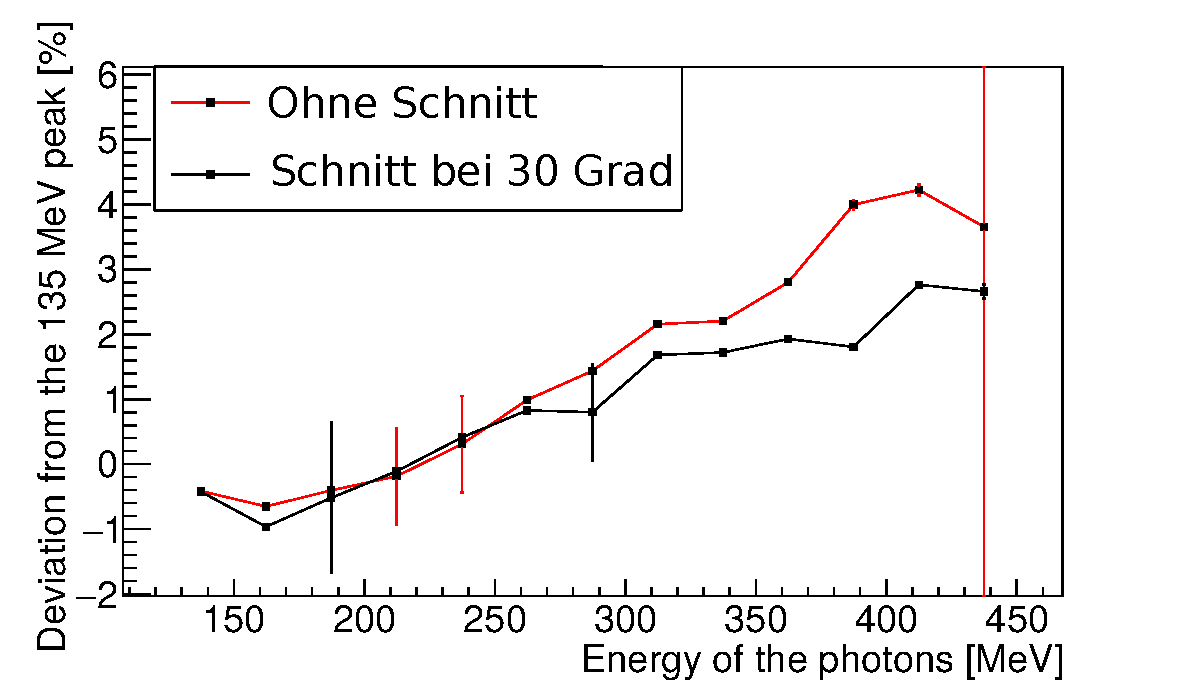
\includegraphics[width=0.75\textwidth]{Pictures/20170405StrahlzeitBothDeviation}
	\caption{Beamtime: With and without considerations of the detectors on the edge of the beam entrance and exit }
\end{figure}	
\end{frame}

\begin{frame}
	\frametitle{Detectors on the Edge}
	\begin{itemize}
	
	\item Simulation
	\item Red:\, \, No additional cut
	
	Black: Neglect the detectors on the edge
		
	\end{itemize}

\begin{figure}
	
	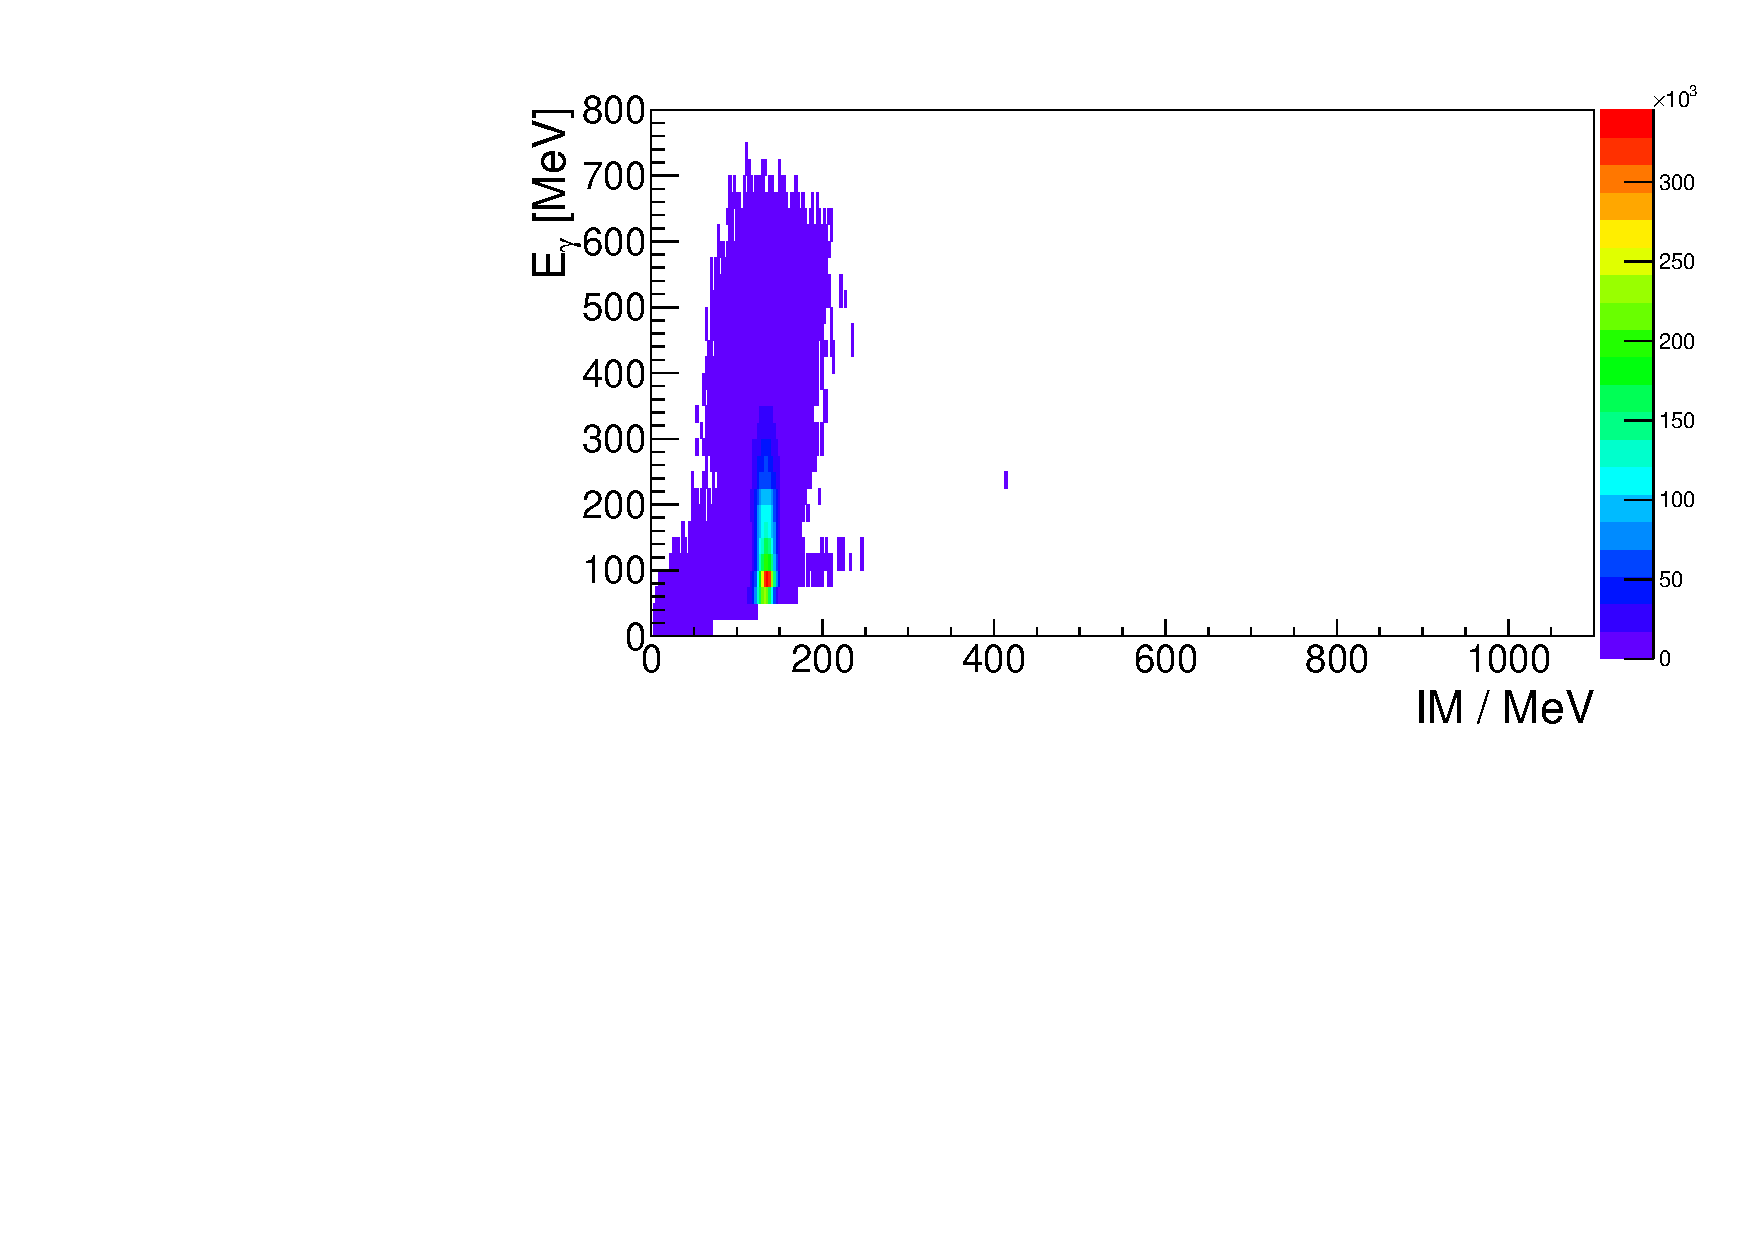
\includegraphics[width=0.50\textwidth]{Pictures/20171904SimNoCut2DHist}
	\hfill
	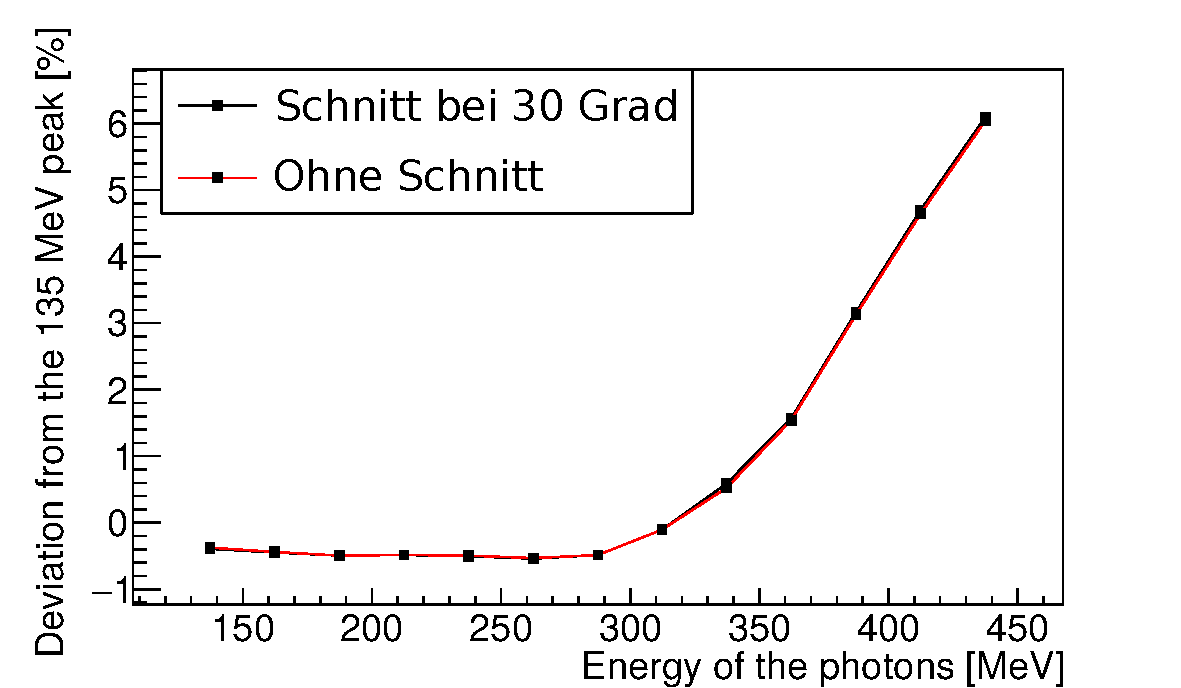
\includegraphics[width=0.50\textwidth]{Pictures/20172804MCBothDeviation}
	\caption{Simulation: Left: Example for the two dimensional histogram with simulated data. Right: Deviation with and without the detectors on the edge}
\end{figure}	
	
\end{frame}
\begin{frame}
	\frametitle{Minimum Opening Angle}
	\begin{itemize}
		\item Simulation
		\item Opening angle $\alpha$ has to be bigger than $30^{\circ}$ degree
		\item $m_{\pi^0}=\sqrt{2 E_1 E_2 (1-\text{cos}(\alpha))}$ with $E_1 \approx E_2$ $\rightarrow E_{max}\approx 250 \, \text{MeV}$
	\end{itemize}

	\begin{figure}
		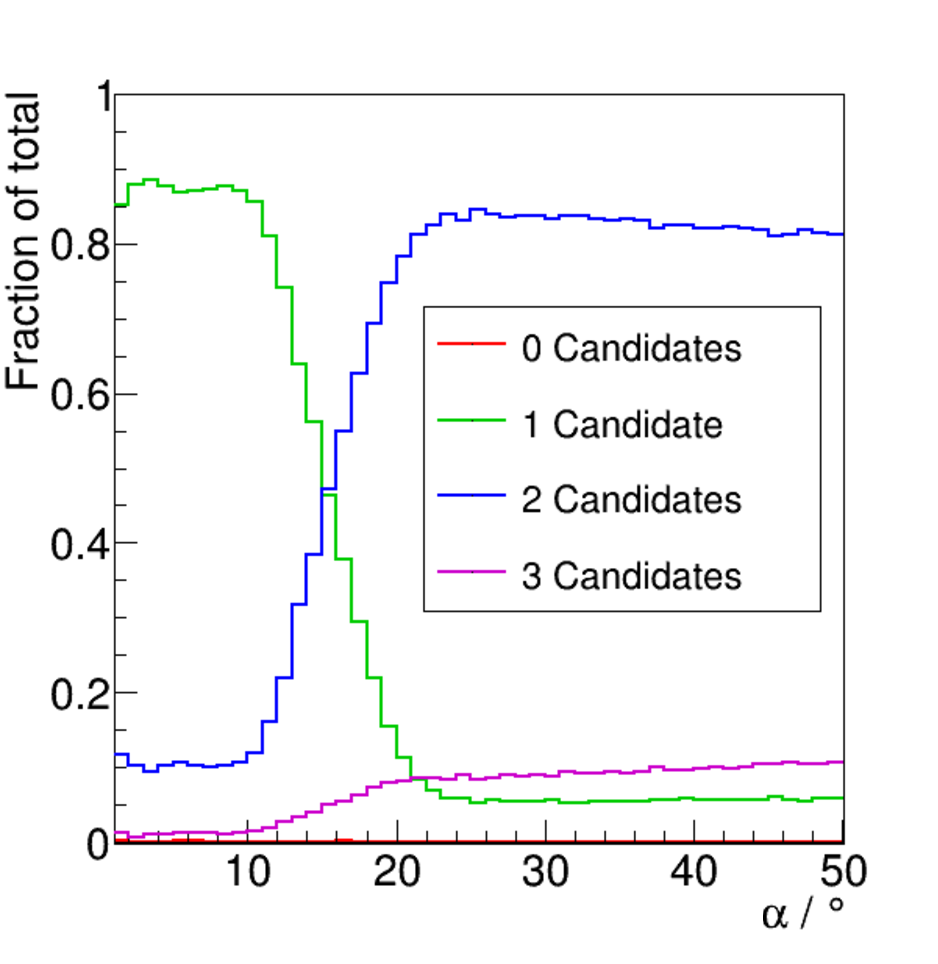
\includegraphics[width=0.35\textwidth]{Pictures/MCClusteringCheck_nCandsOpAng}
		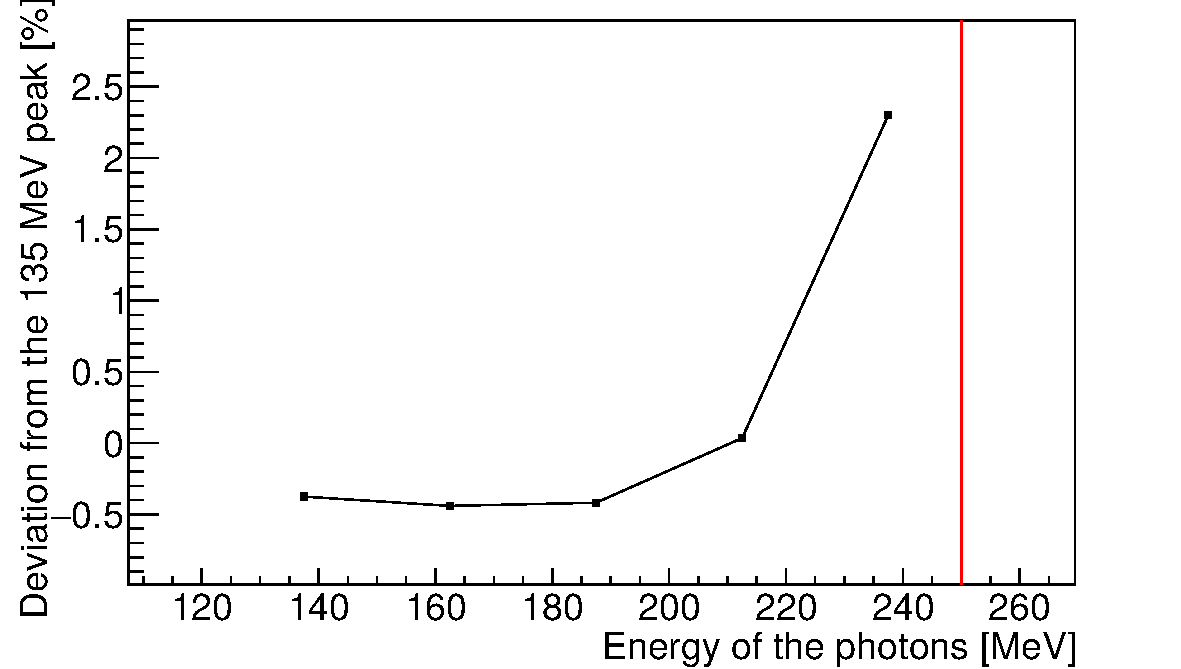
\includegraphics[width=0.50\textwidth]{Pictures/20170505MinAngle30Deviation}
		\caption{Left: Number of reconstructed candidates for different opening angles. Right: Deviation with $\alpha > 30 \, \text{MeV}$ }
	\end{figure}
	
\end{frame}

\begin{frame}
	\frametitle{Isotropic Decay}
	\begin{itemize}
		\item Simulation
		\item $\pi^0$ decay in the origin of the target
		\item $\pi^0$ are boosted isotropic with an energy of $ 1420\, \text{MeV}$ to $1580\, \text{MeV}$
	\end{itemize}
	
	\begin{figure}
		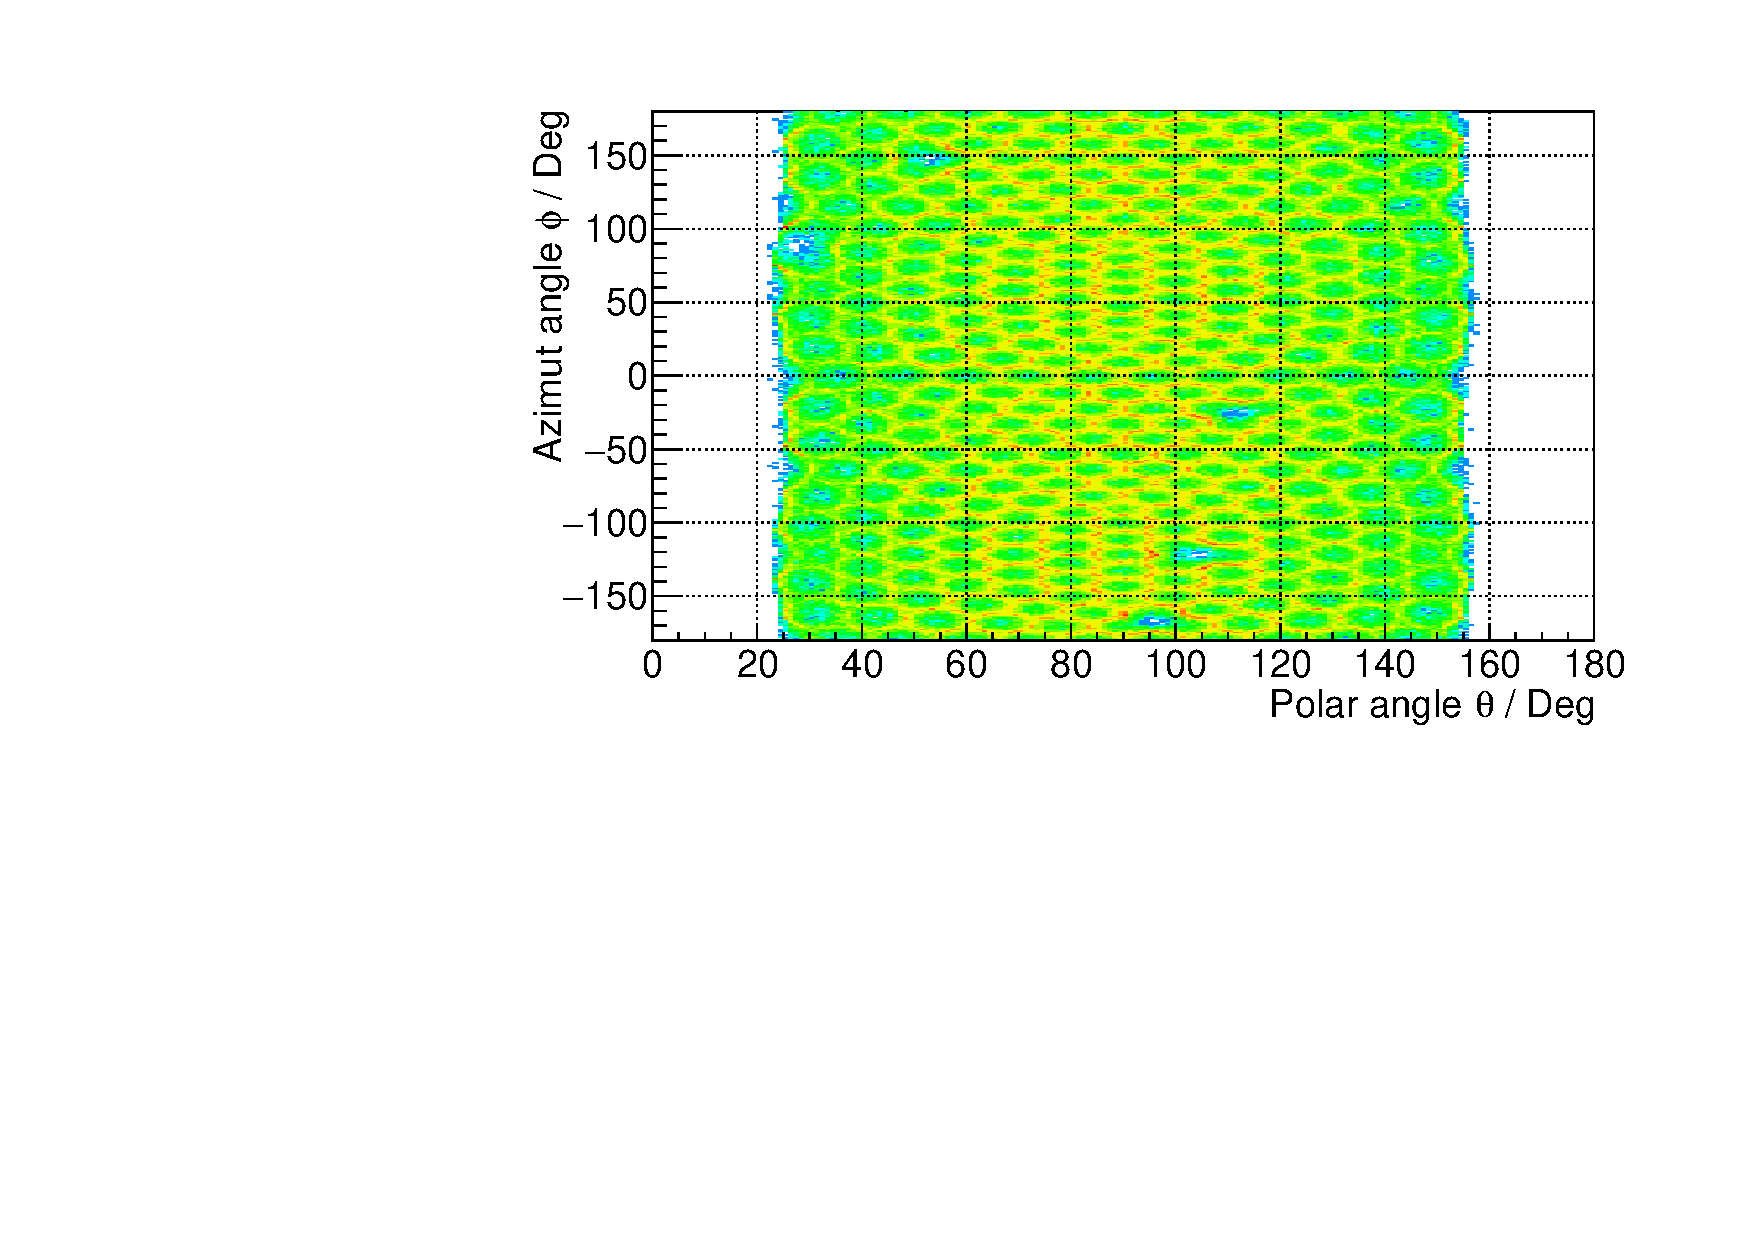
\includegraphics[width=0.50\textwidth]{Pictures/20171204DistributionPhotonUrsprungIsotrop}
		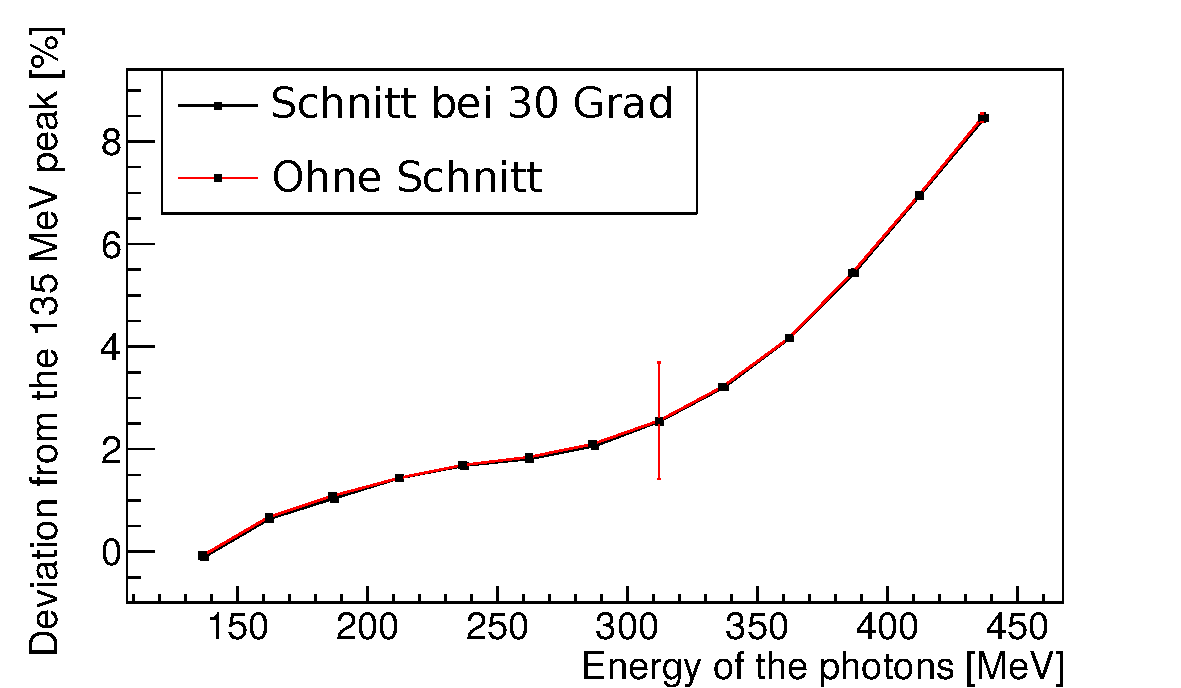
\includegraphics[width=0.50\textwidth]{Pictures/20172804IsotropUrpsprungDeviation}
		\caption{Simulation: Isotropic decay in the origin of the target}
	\end{figure}
\end{frame}

\begin{frame}
	\frametitle{$z$-Vertex Dependency}
	\begin{itemize}
		\item Simulation
		\item Neglect the detectors on the edge
		\item Devide the target in smaller sections of $1\,\text{cm}$
	\end{itemize}


\begin{figure}
	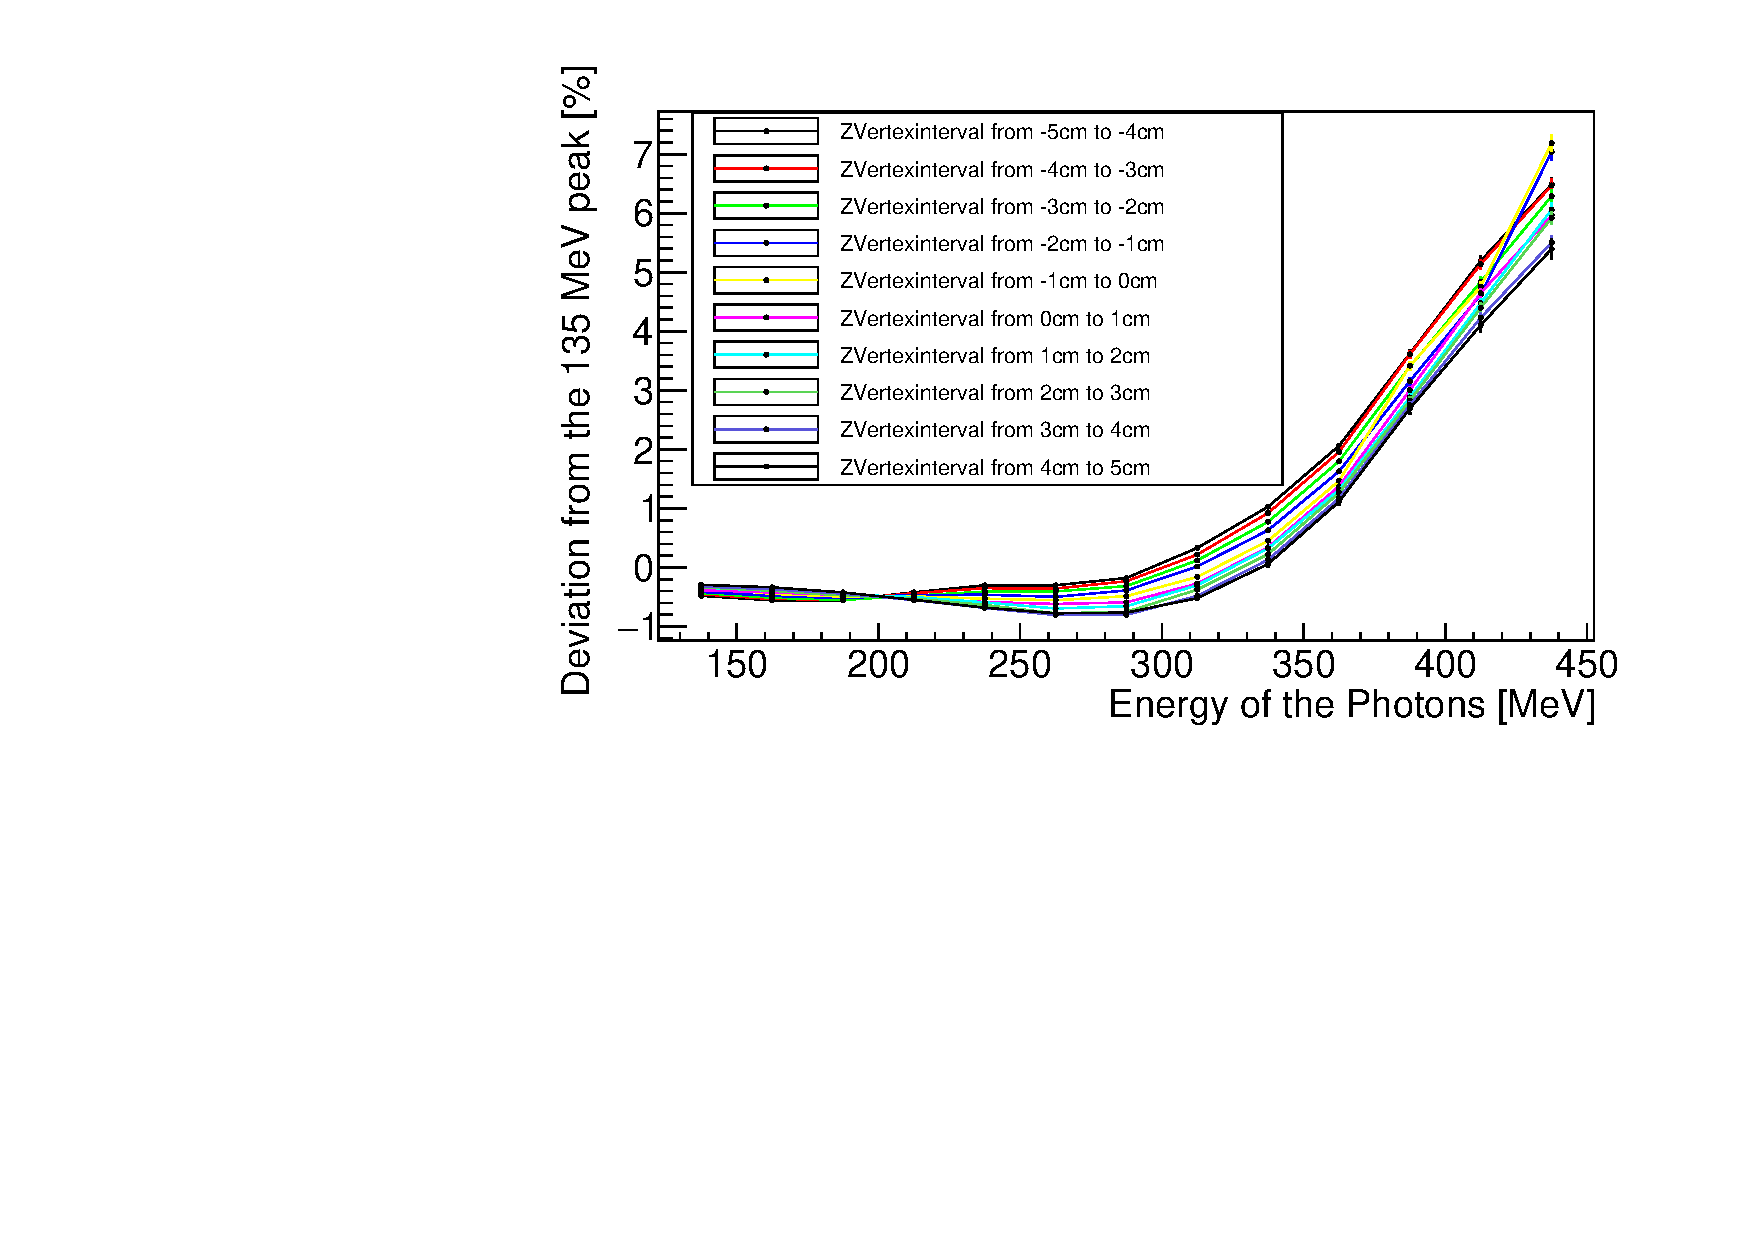
\includegraphics[width=0.750\textwidth]{Pictures/20172804MCZVertexDeviation}
	\caption{Simulation: Deviations for different $z$-Vertices}
\end{figure}

\end{frame}

\begin{frame}
	\frametitle{Angle between Generated and Reconstructed Candidates }

\begin{itemize}
	\item Simulation
	\item The angle between generated and reconstructed candidate is calculated
\end{itemize}

\begin{figure}
	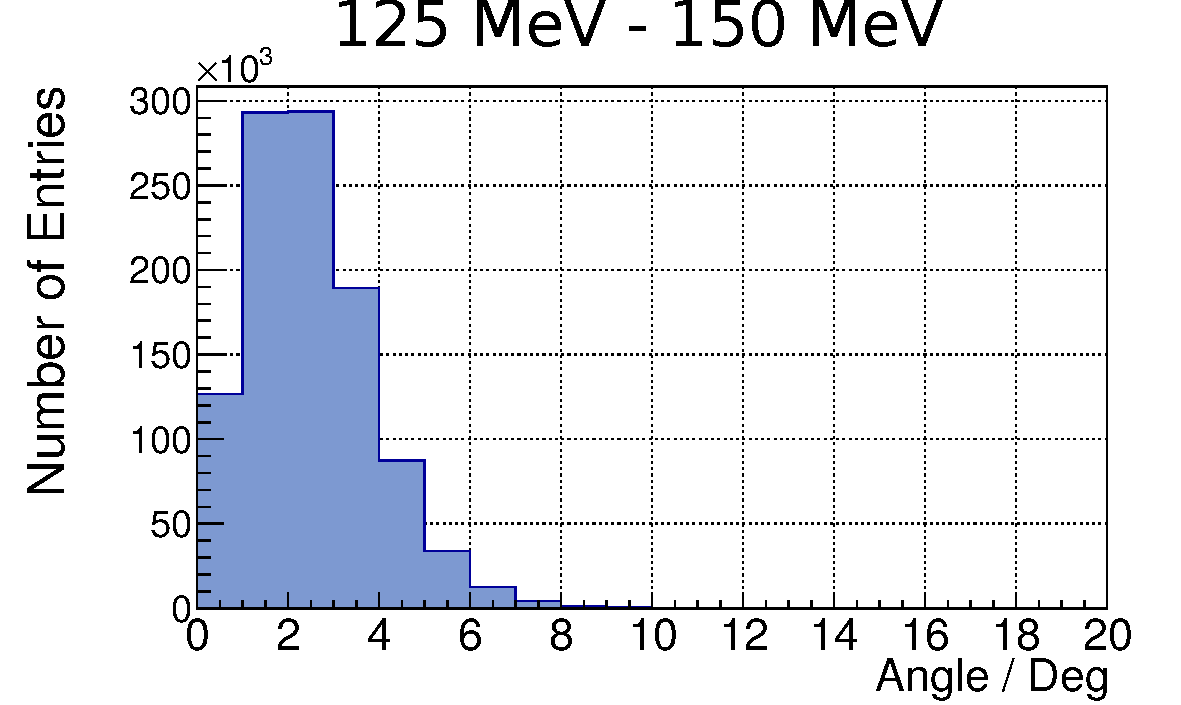
\includegraphics[width=0.5\textwidth]{Pictures/20172604AngleRegGen100-125MeV}
	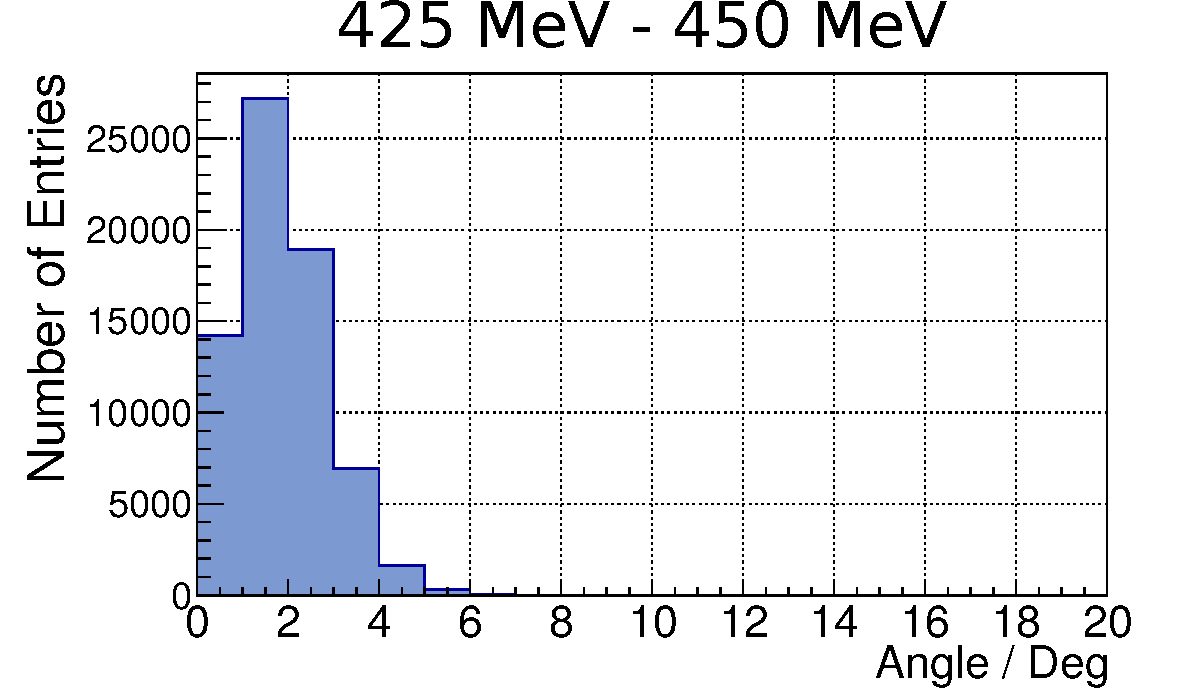
\includegraphics[width=0.5\textwidth]{Pictures/20172604AngleRegGen400-425MeV}
	\caption{Simulation: Angle between gen. and rec. candidates. Left: Photon energy between $125\,\text{MeV}$ and $150\,\text{MeV}$. Right: Photon energy between $425\,\text{MeV} $ and $ 450\,\text{MeV}$}
\end{figure}

\end{frame}

\begin{frame}
	\frametitle{Difference between Generated and Reconstructed Opening Angle}
	
	\begin{itemize}
		\item Simulation
		\item $\Delta \alpha = \alpha_{rec}-\alpha_{gen}$
	\end{itemize}
\begin{figure}
	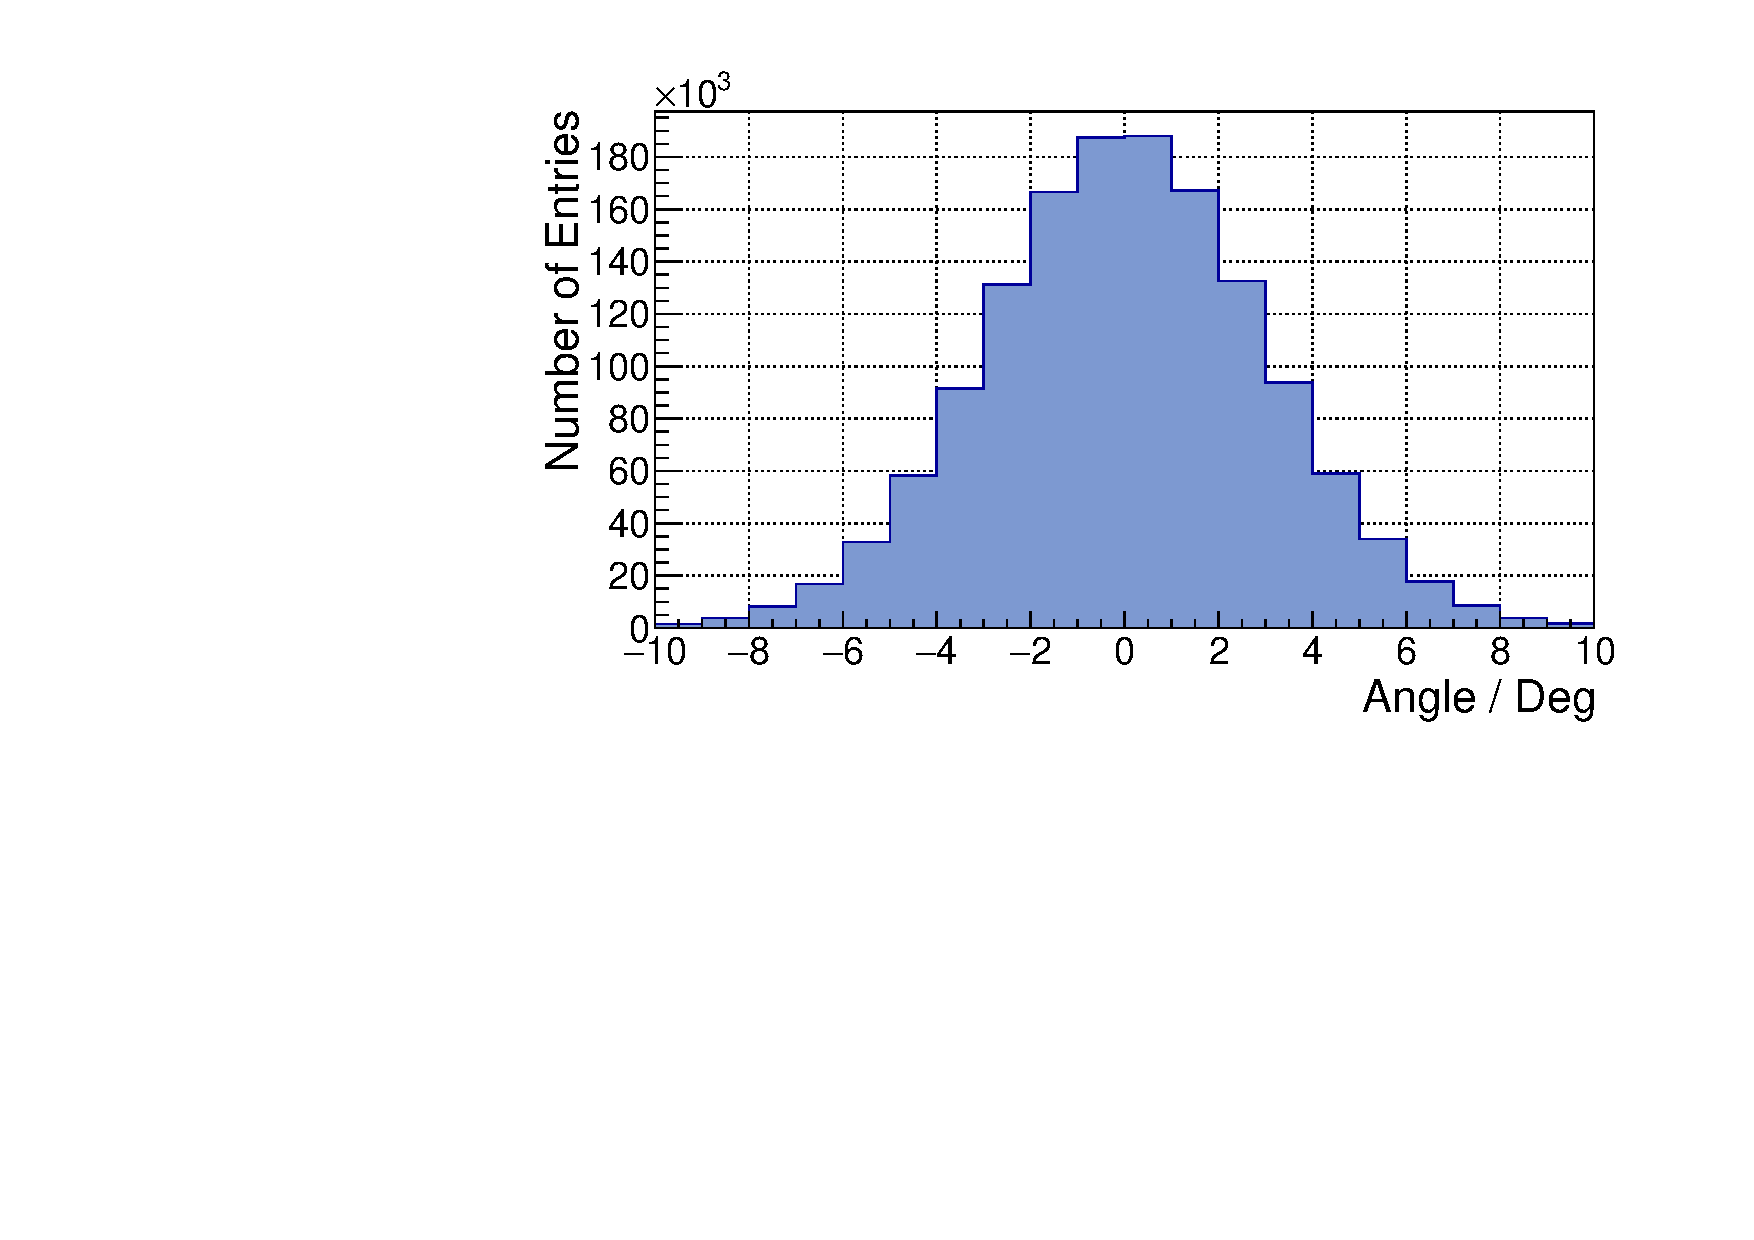
\includegraphics[width=0.5\textwidth]{Pictures/20172704MCDeviationOpeningAngle125MeV}
	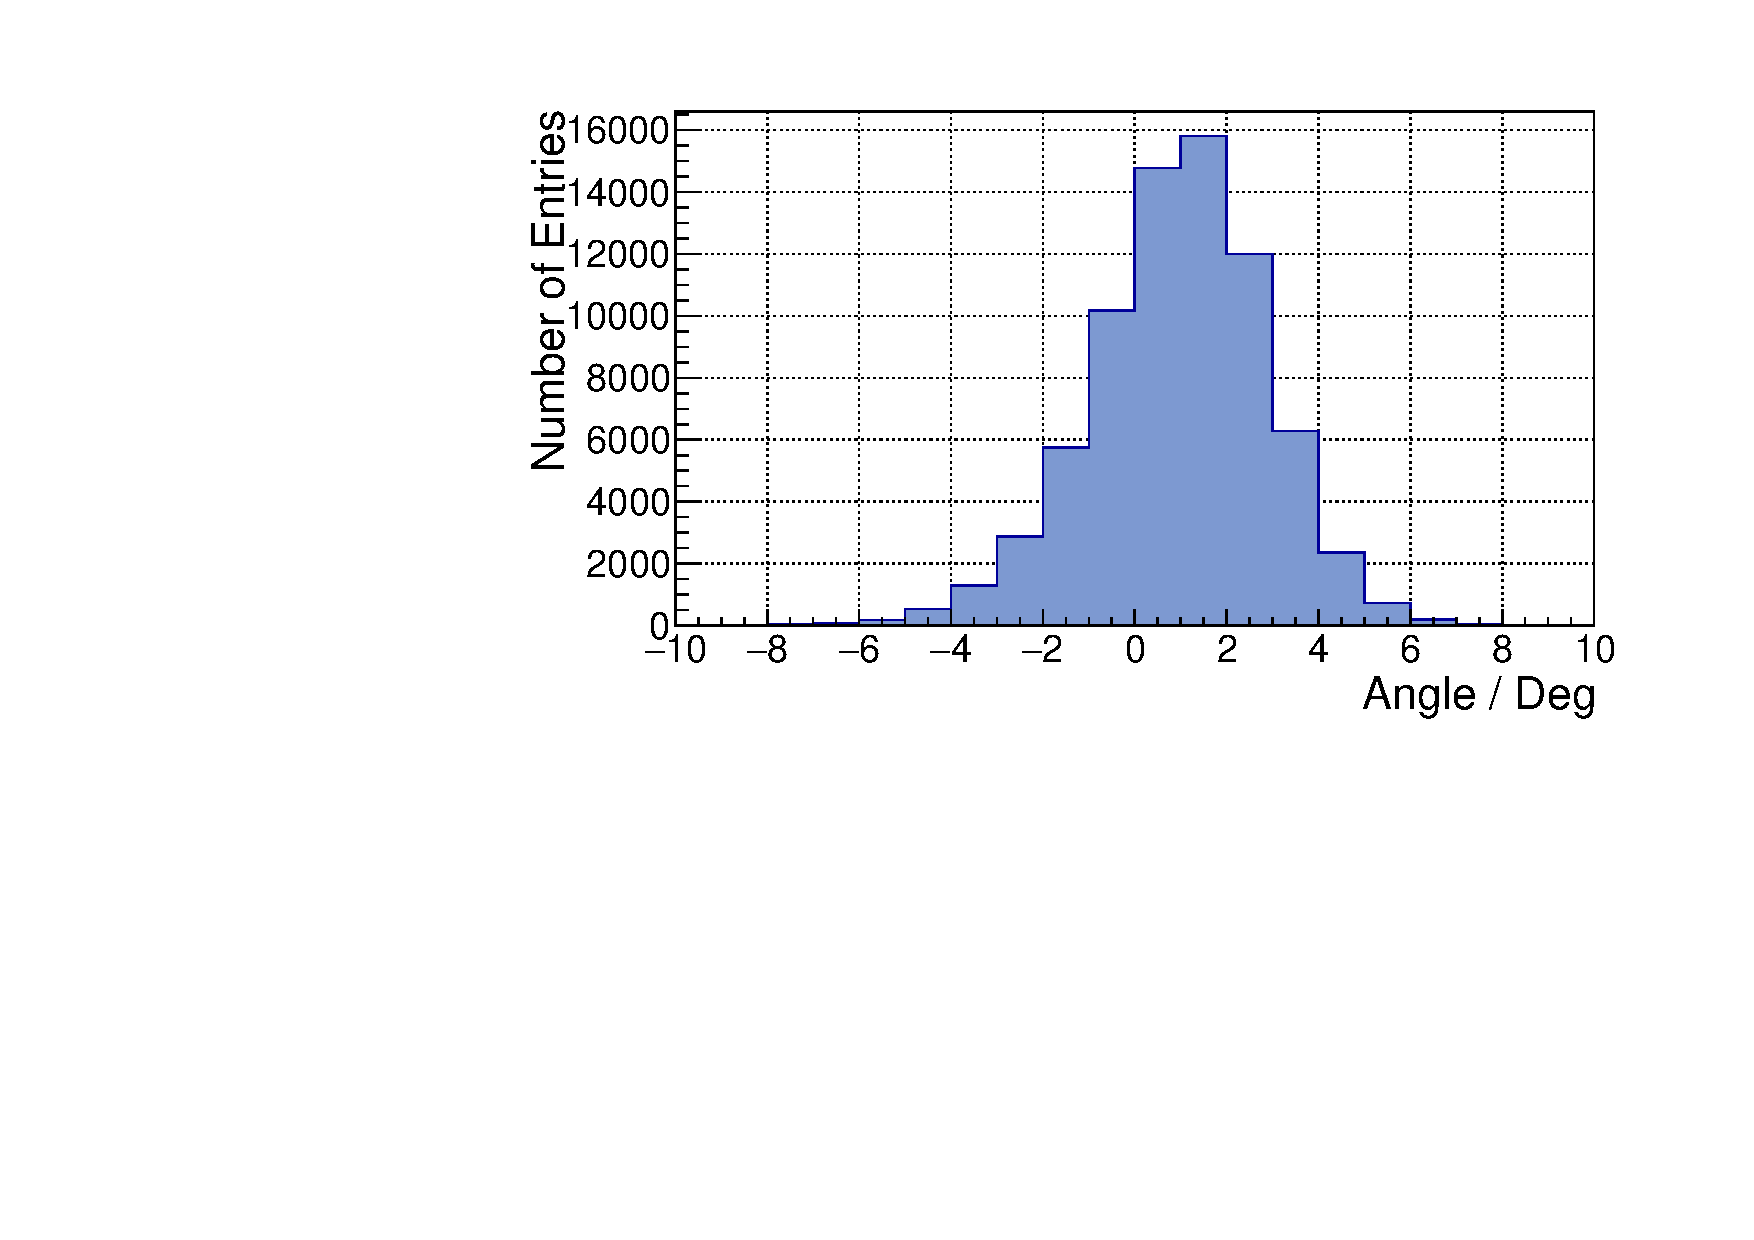
\includegraphics[width=0.5\textwidth]{Pictures/20172704MCDeviationOpeningAngle400MeV}
\caption{Simulation: $\Delta \alpha$ for different photon energies. Left $125\,\text{MeV}$ to $150\,\text{MeV}$. Right from $425\,\text{MeV}$ to $450\,\text{MeV}$}
\end{figure}


\end{frame}

\begin{frame}
	\frametitle{$\Delta \alpha$ for Different $z$-Vertices}
	\begin{itemize}
		\item Simulation
		\item $\Delta \alpha$ for different $z$-Vertices
	\end{itemize}

\begin{figure}
	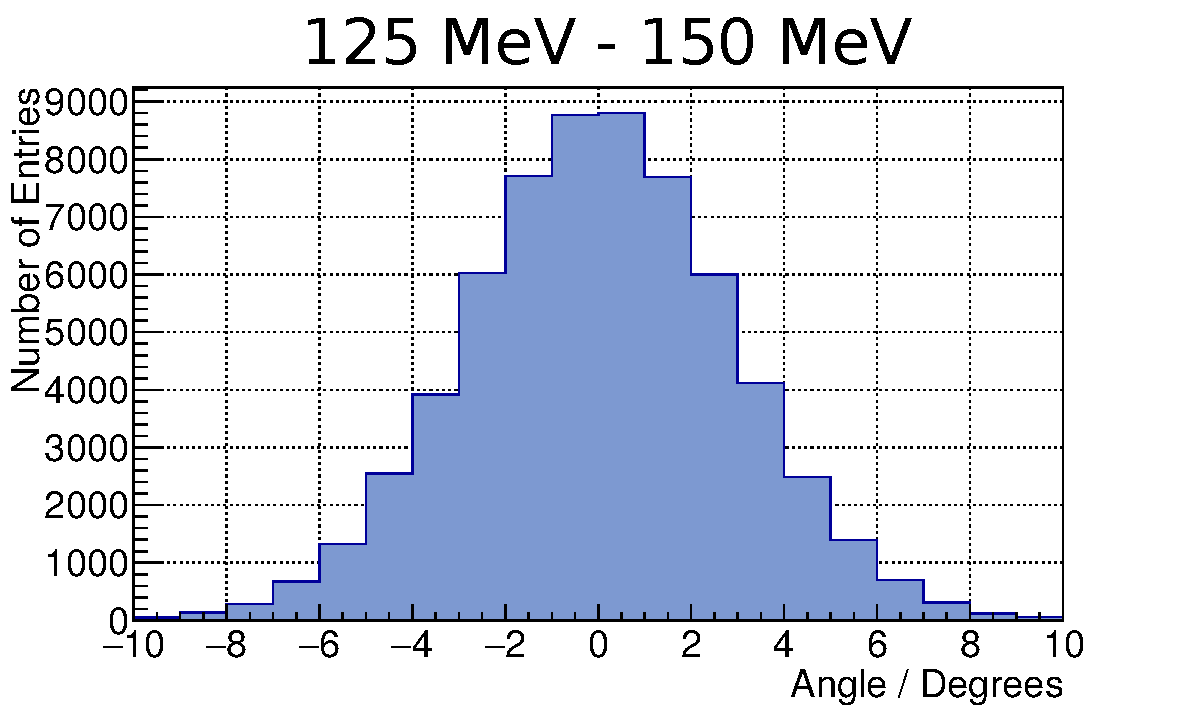
\includegraphics[width=0.35\textwidth]{Pictures/20170205DiffOeffZVertex-4_125MeV}
	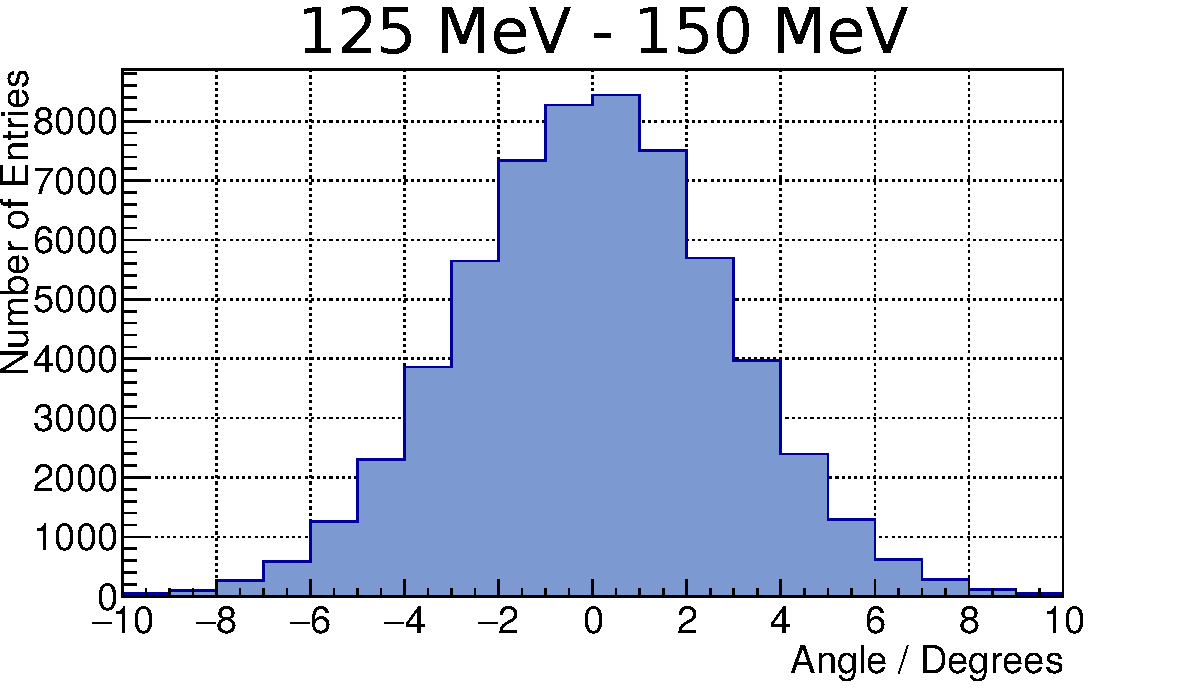
\includegraphics[width=0.35\textwidth]{Pictures/20170205DiffOeffZVertexUrsprung135MeV}	
	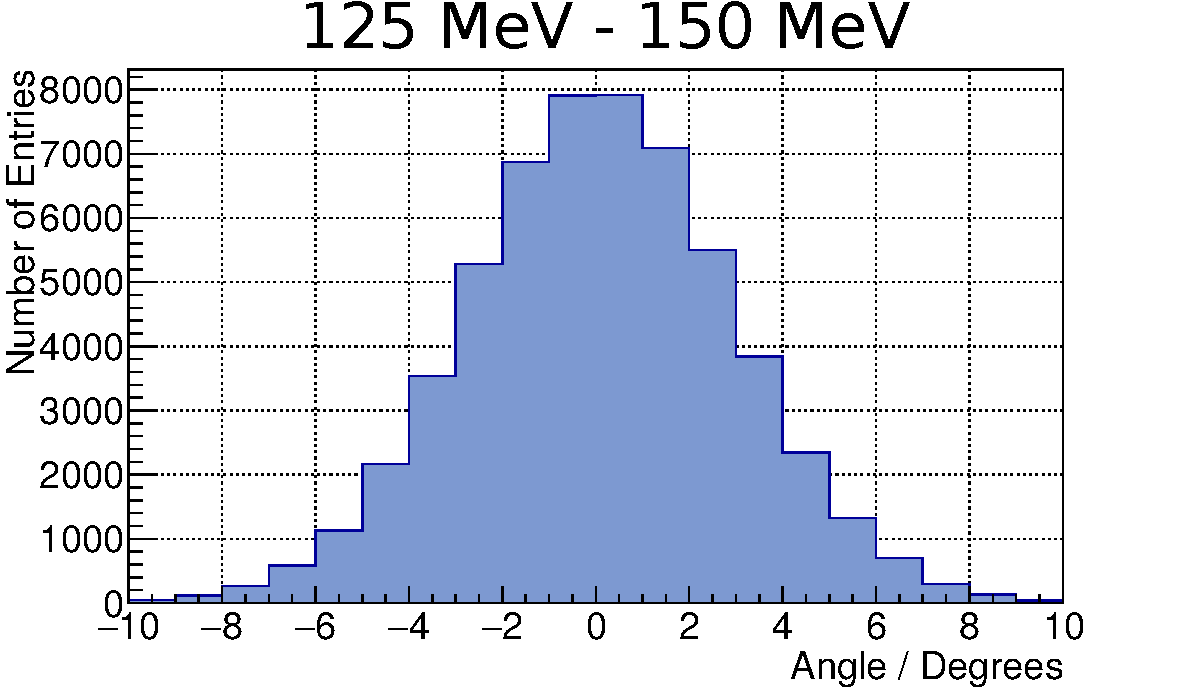
\includegraphics[width=0.35\textwidth]{Pictures/20170205DiffOeffZVertex+4_125MeV}	

	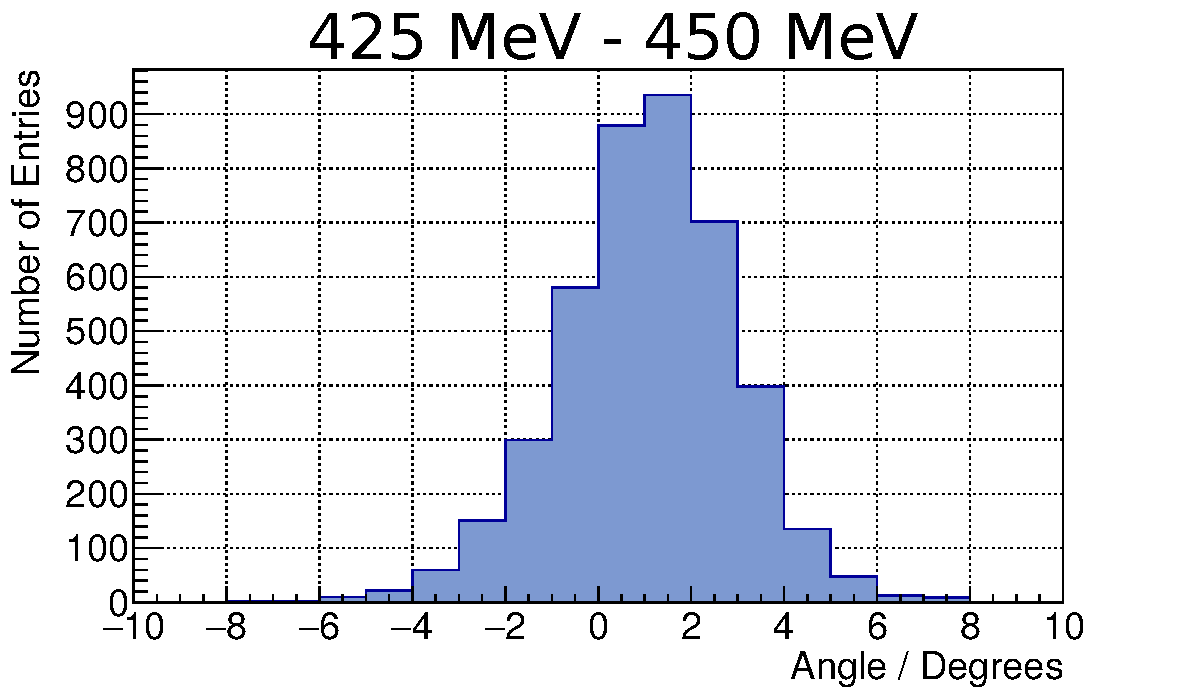
\includegraphics[width=0.35\textwidth]{Pictures/20170205DiffOeffZVertex-4_425MeV}
	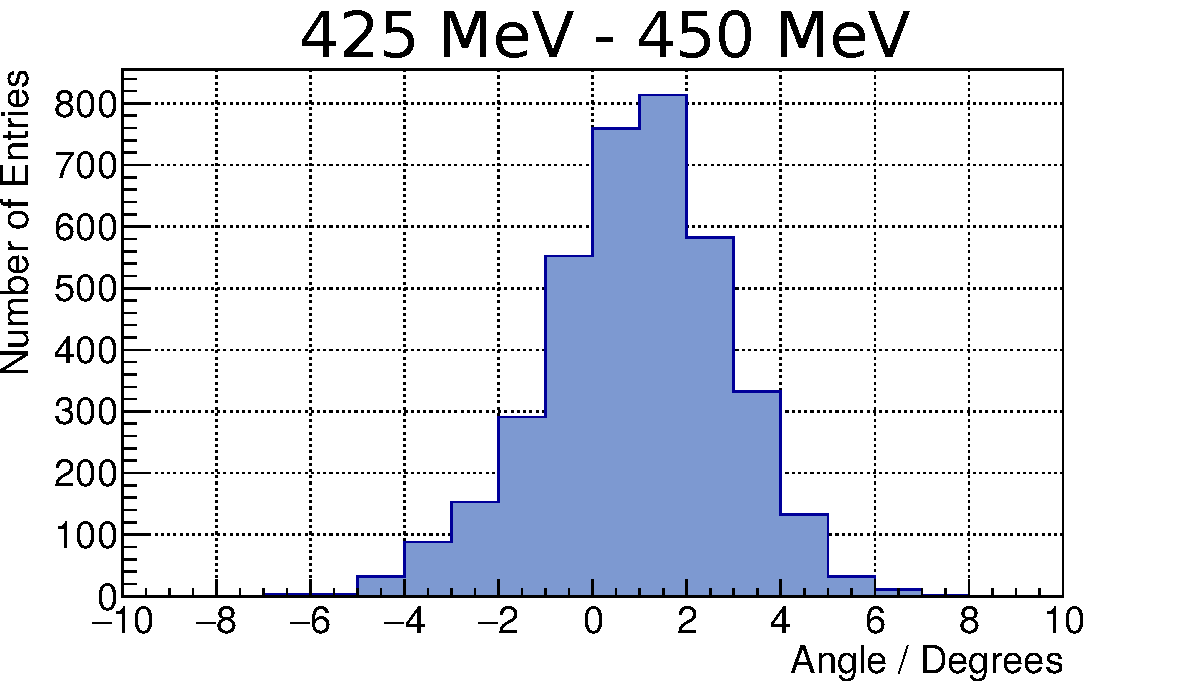
\includegraphics[width=0.35\textwidth]{Pictures/20170205DiffOeffZVertexUrsprung425MeV}
	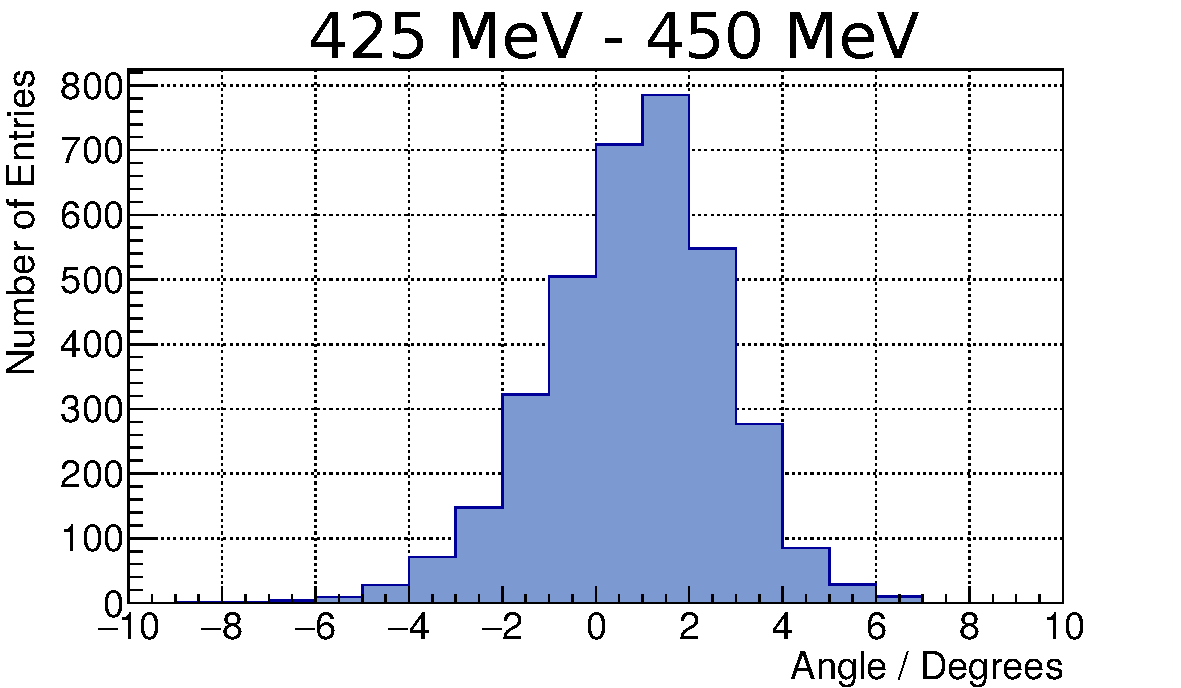
\includegraphics[width=0.35\textwidth]{Pictures/20170205DiffOeffZVertex+4_425MeV}	
	\caption{Simulation: $\Delta \alpha$ for different photon energies. Decay at different $z$-Vertices}
\end{figure}
	
\end{frame}




\section{Further Results}
\begin{frame}
	\frametitle{Hot Crystals}
	\begin{itemize}
		\item Beamtime October 2014
		\item Photon energy between $0\,\text{MeV}$ and $100\,\text{MeV}$
	\end{itemize}
	\begin{figure}
		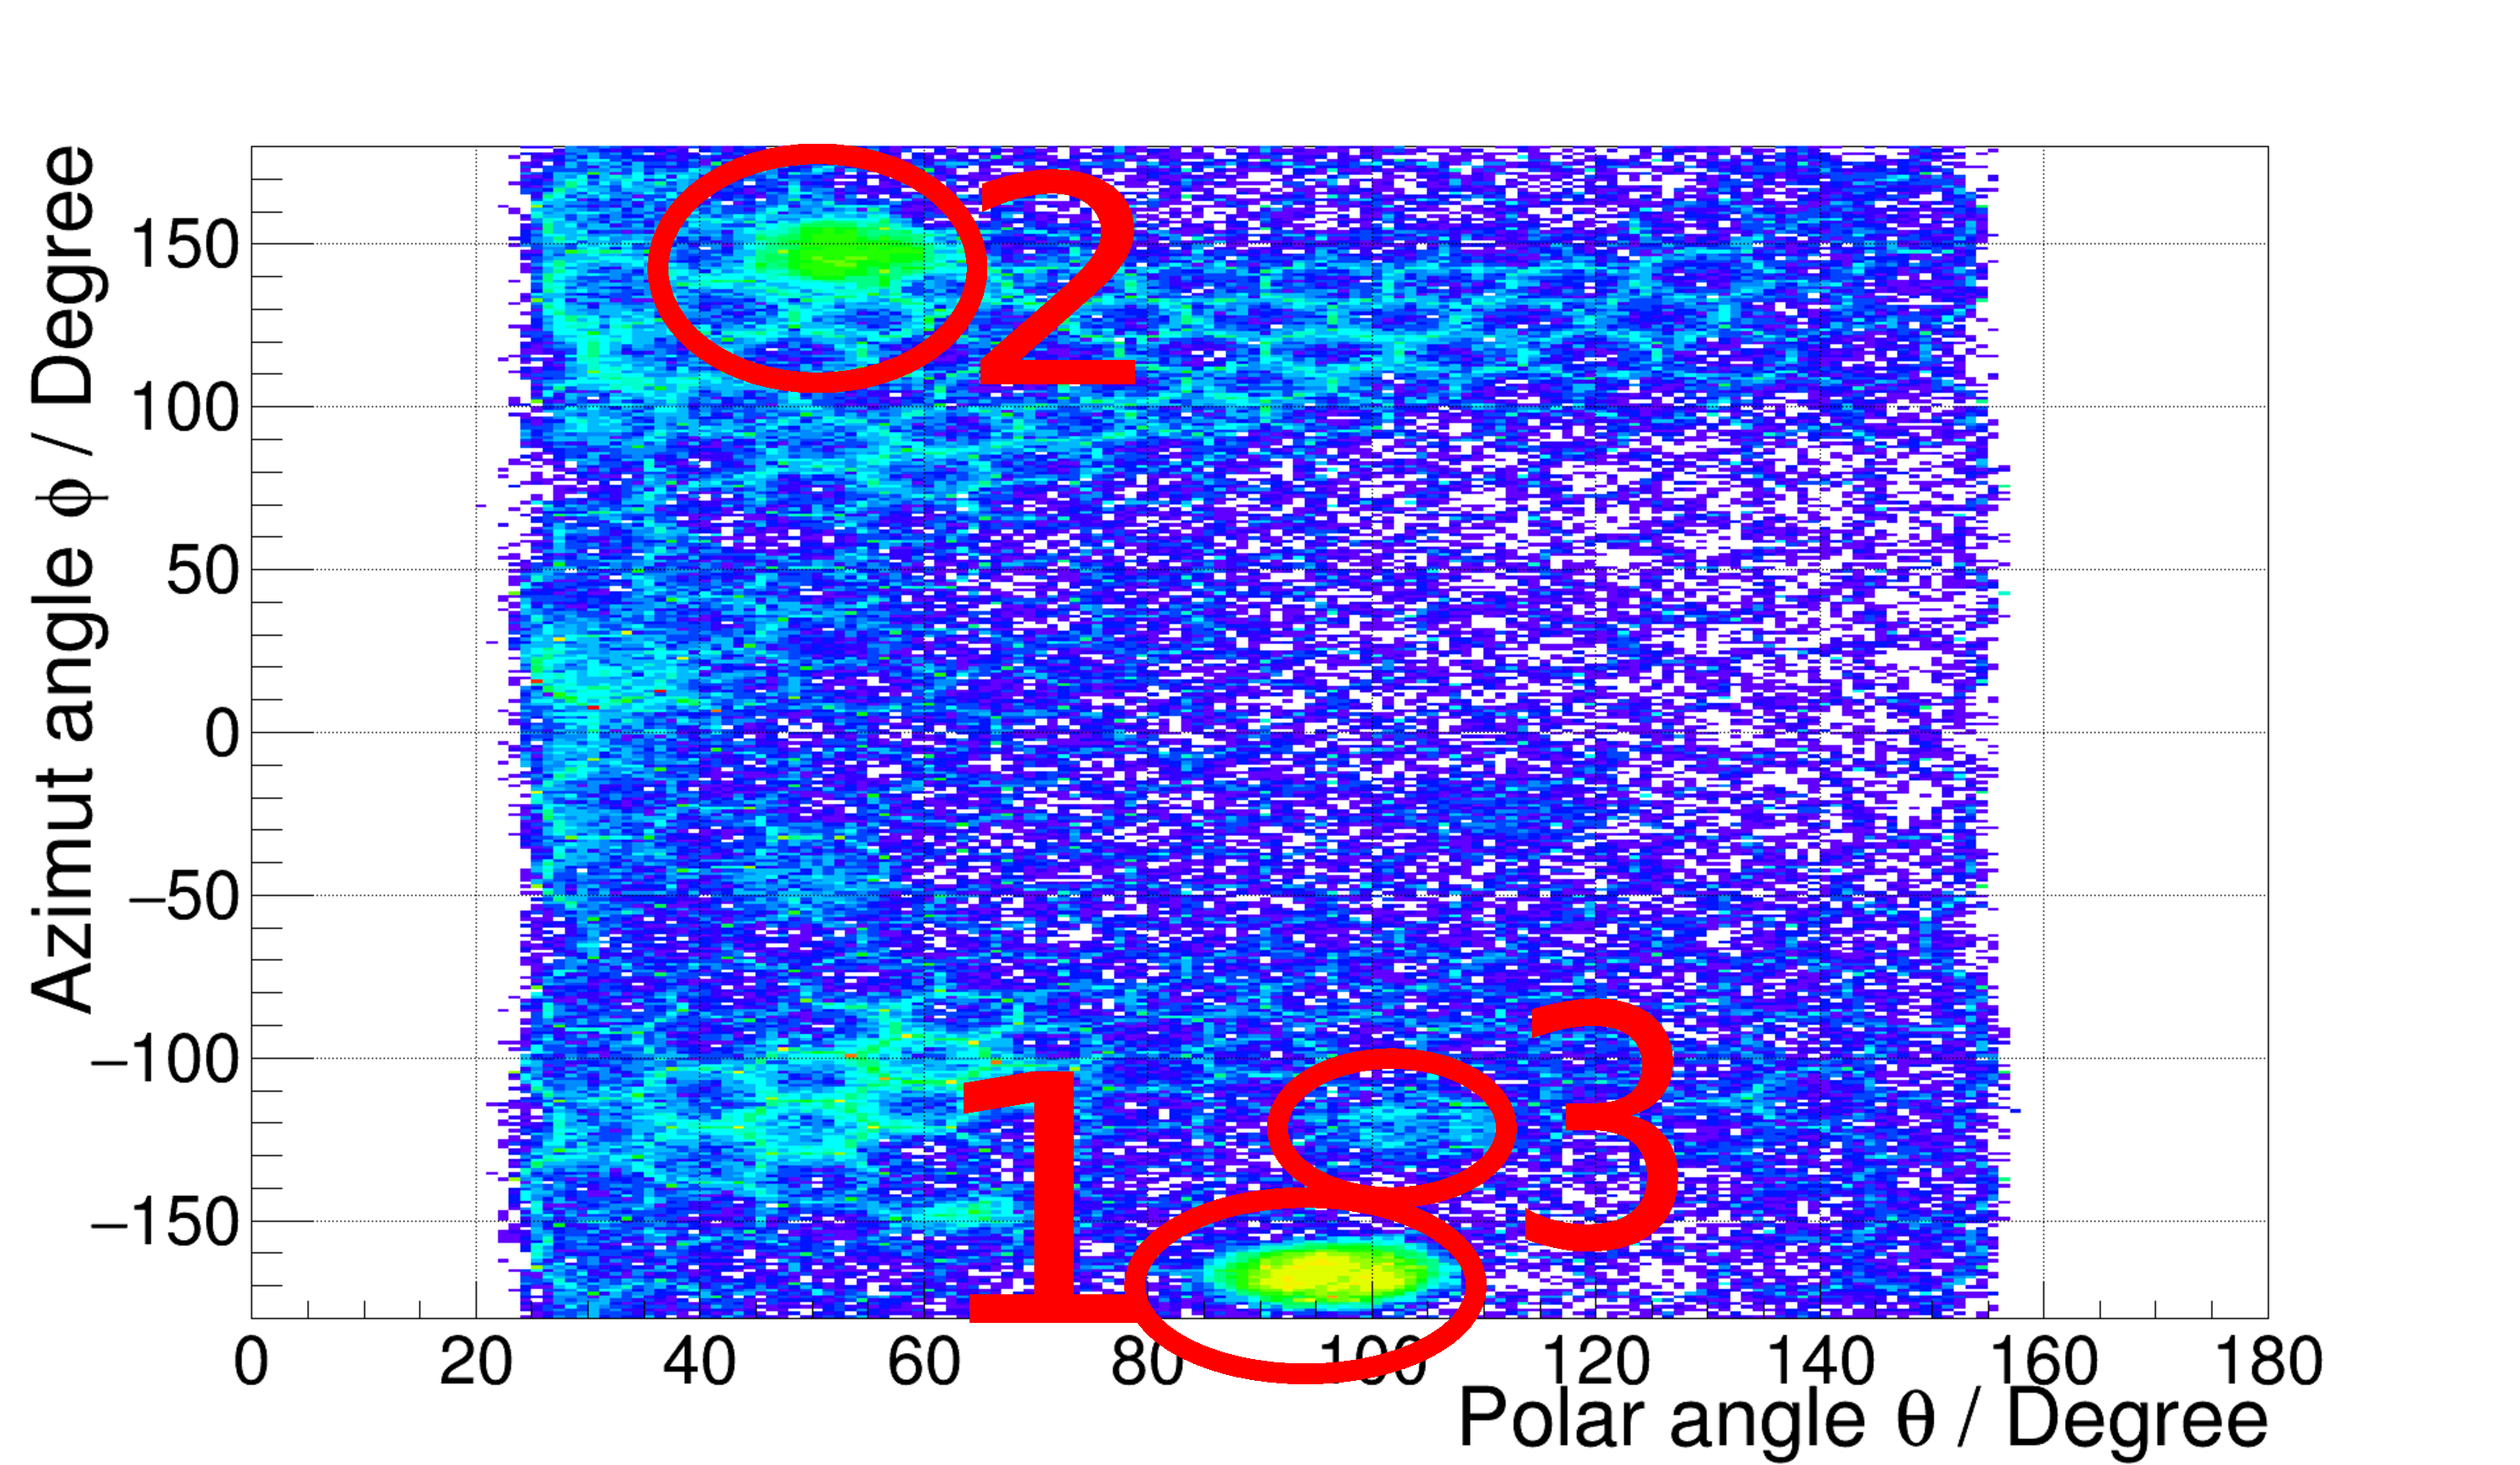
\includegraphics[width=0.50\textwidth]{Pictures/20172104StrahlzeitClusterSize0Marker}
		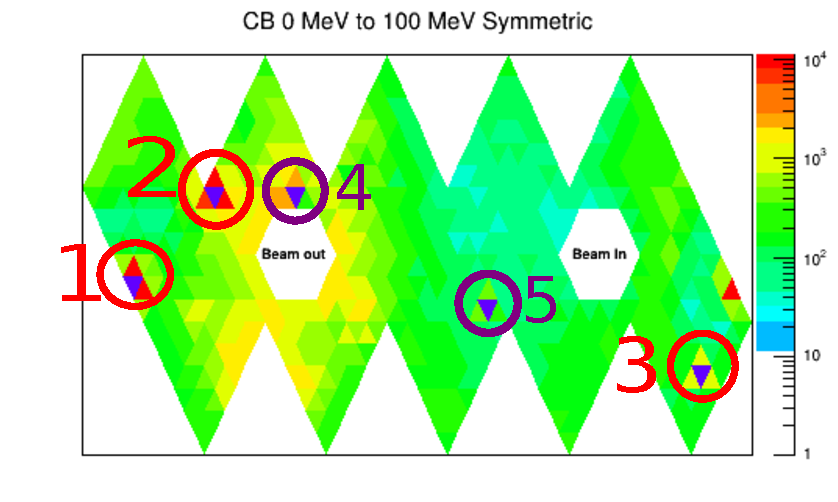
\includegraphics[width=0.50\textwidth]{Pictures/20172104StrahlzeitClusterSize0MarkerMap}
		\caption{Beamtime: Marked are Hot and known Dead Crystals }
	\end{figure}
	\begin{table}
	\captionof{table}{Beamtime: Element No. and No. in figure}
	\scalebox{0.7}{
	\begin{tabular}{lccccc}
		Number in the figures & 1 & 2 & 3 & 4 & 5 \\
		Element Number & 549 & 565 & 597 & 677 & 265 
		
	\end{tabular}}
	\end{table}
\end{frame}

\begin{frame}
	\frametitle{Hot Crystals and Clustersize $>$ 3}
	\begin{itemize}
		\item Beamtime October 2014
		\item Photon energy between $0\,\text{MeV}$ and $100\,\text{MeV}$
		\item Clustersize $>$ 3
	\end{itemize}

\begin{figure}
	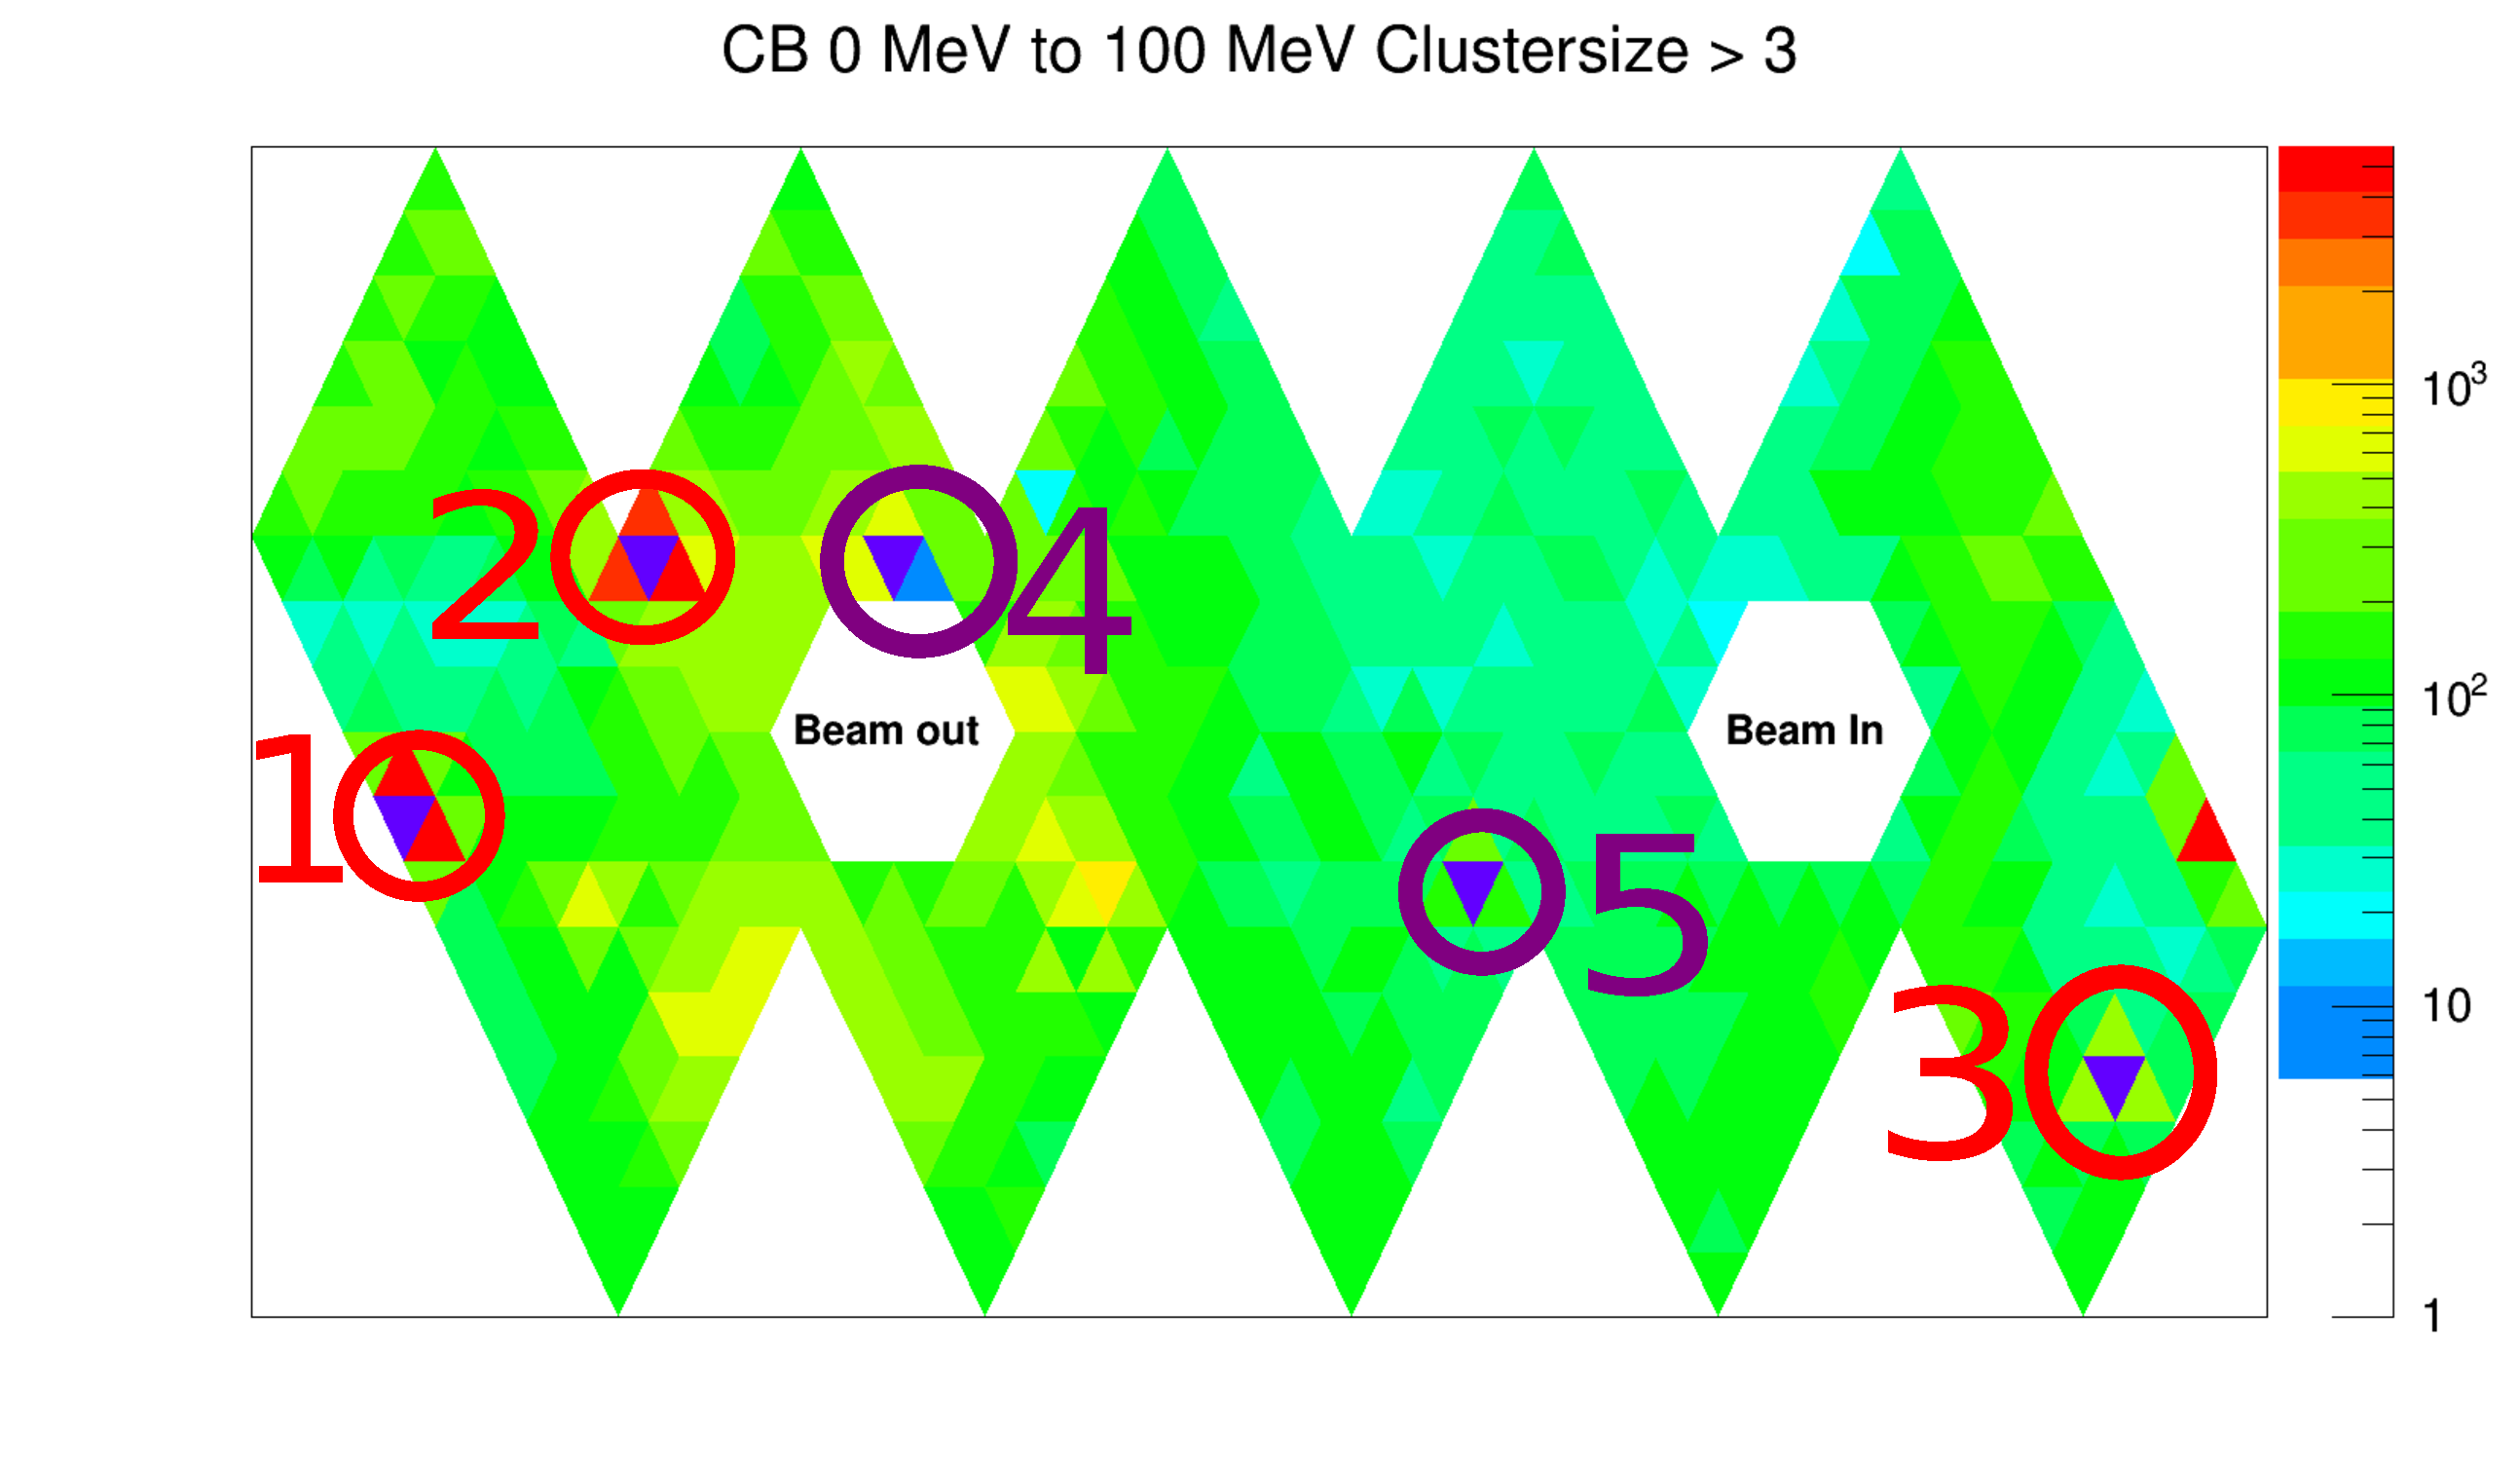
\includegraphics[width=0.75\textwidth]{Pictures/20172404Clustersize3Map100MeV}
	\caption{Beamtime: Marked are Dead and Hot Crystals. The Clustersize must be bigger than 3}
\end{figure}

\end{frame}

\begin{frame}
	\frametitle{Hot Crystals for Higher Energies}
	\begin{itemize}
		\item Beamtime October 2014
		\item Photon energy between $300\,\text{MeV}$ and $400\,\text{MeV}$
	\end{itemize}
\begin{figure}
	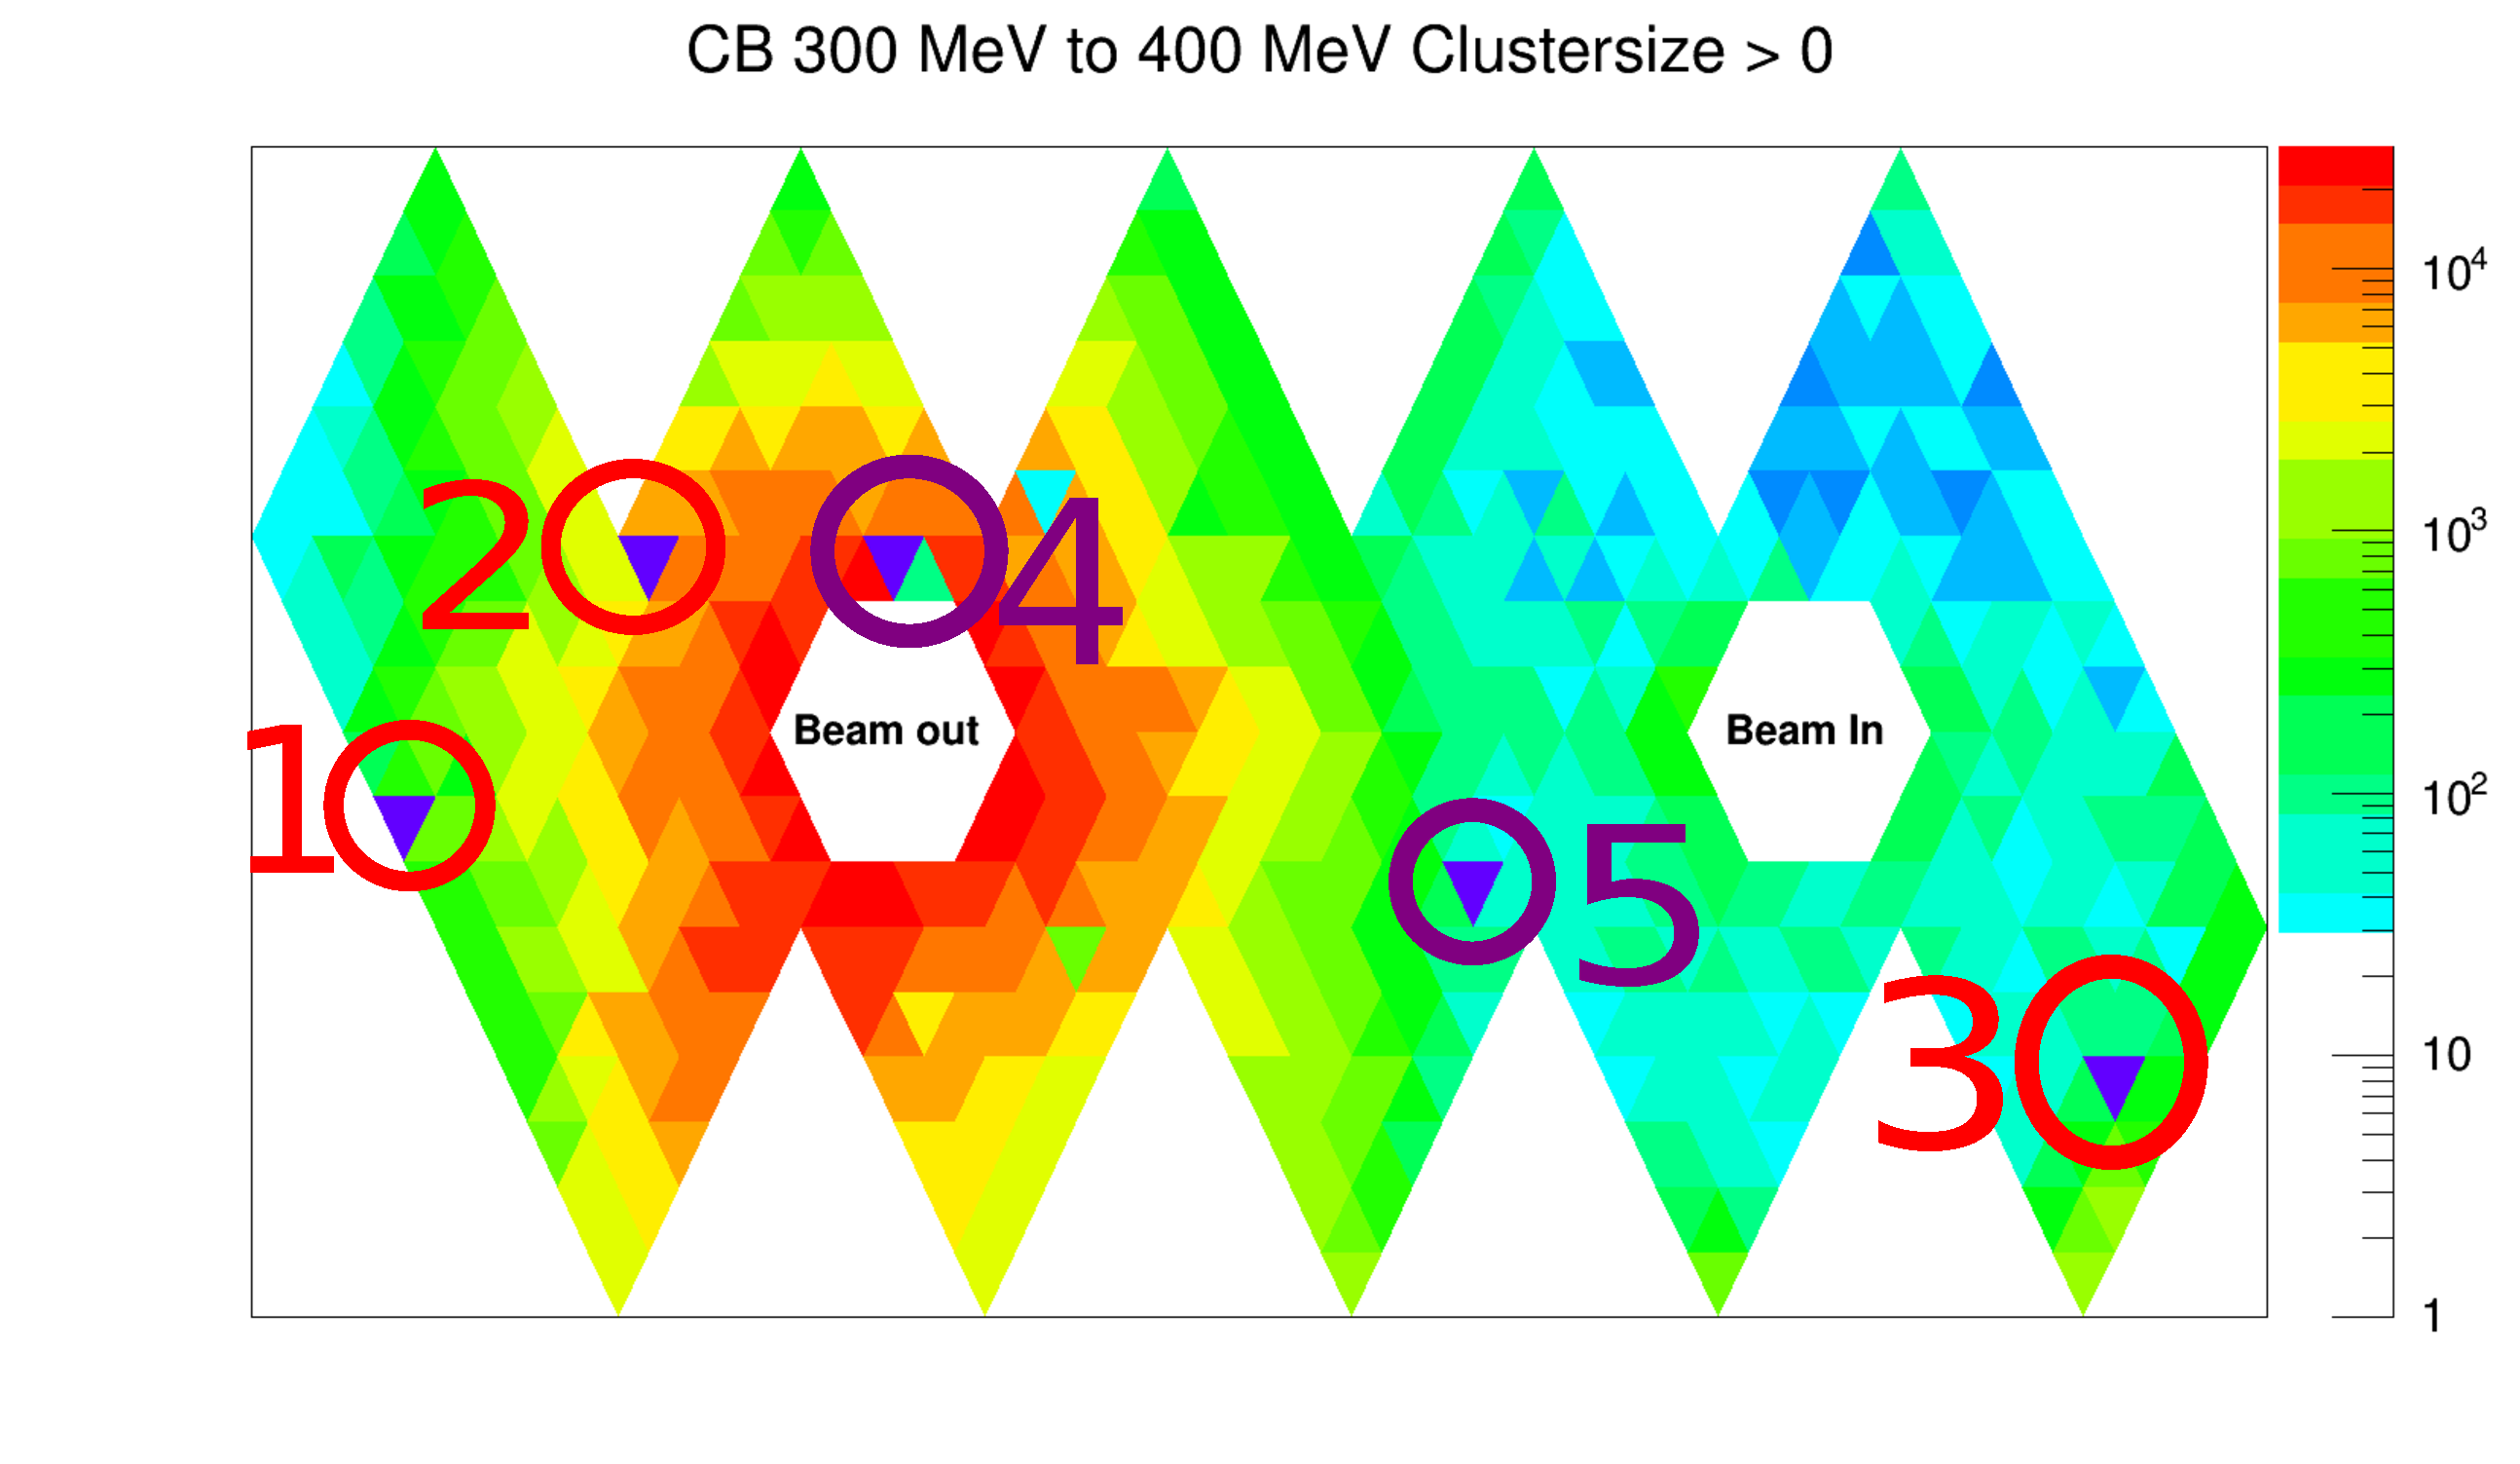
\includegraphics[width=0.75\textwidth]{Pictures/20172404Clustersize0Map400MeV}
	\caption{Beamtime: Marked are Dead and Hot Crystals for high energies}
\end{figure}


\end{frame}

\begin{frame}
	\frametitle{Dead Crystals}
	\begin{itemize}
		\item Beamtime October 2014
		\item Photon energy between $300\,\text{MeV}$ and $400\,\text{MeV}$
	\end{itemize}



	\begin{figure}
		\centering
		\begin{minipage}[t]{.6\textwidth}
			\centering
			\vspace{0pt}
			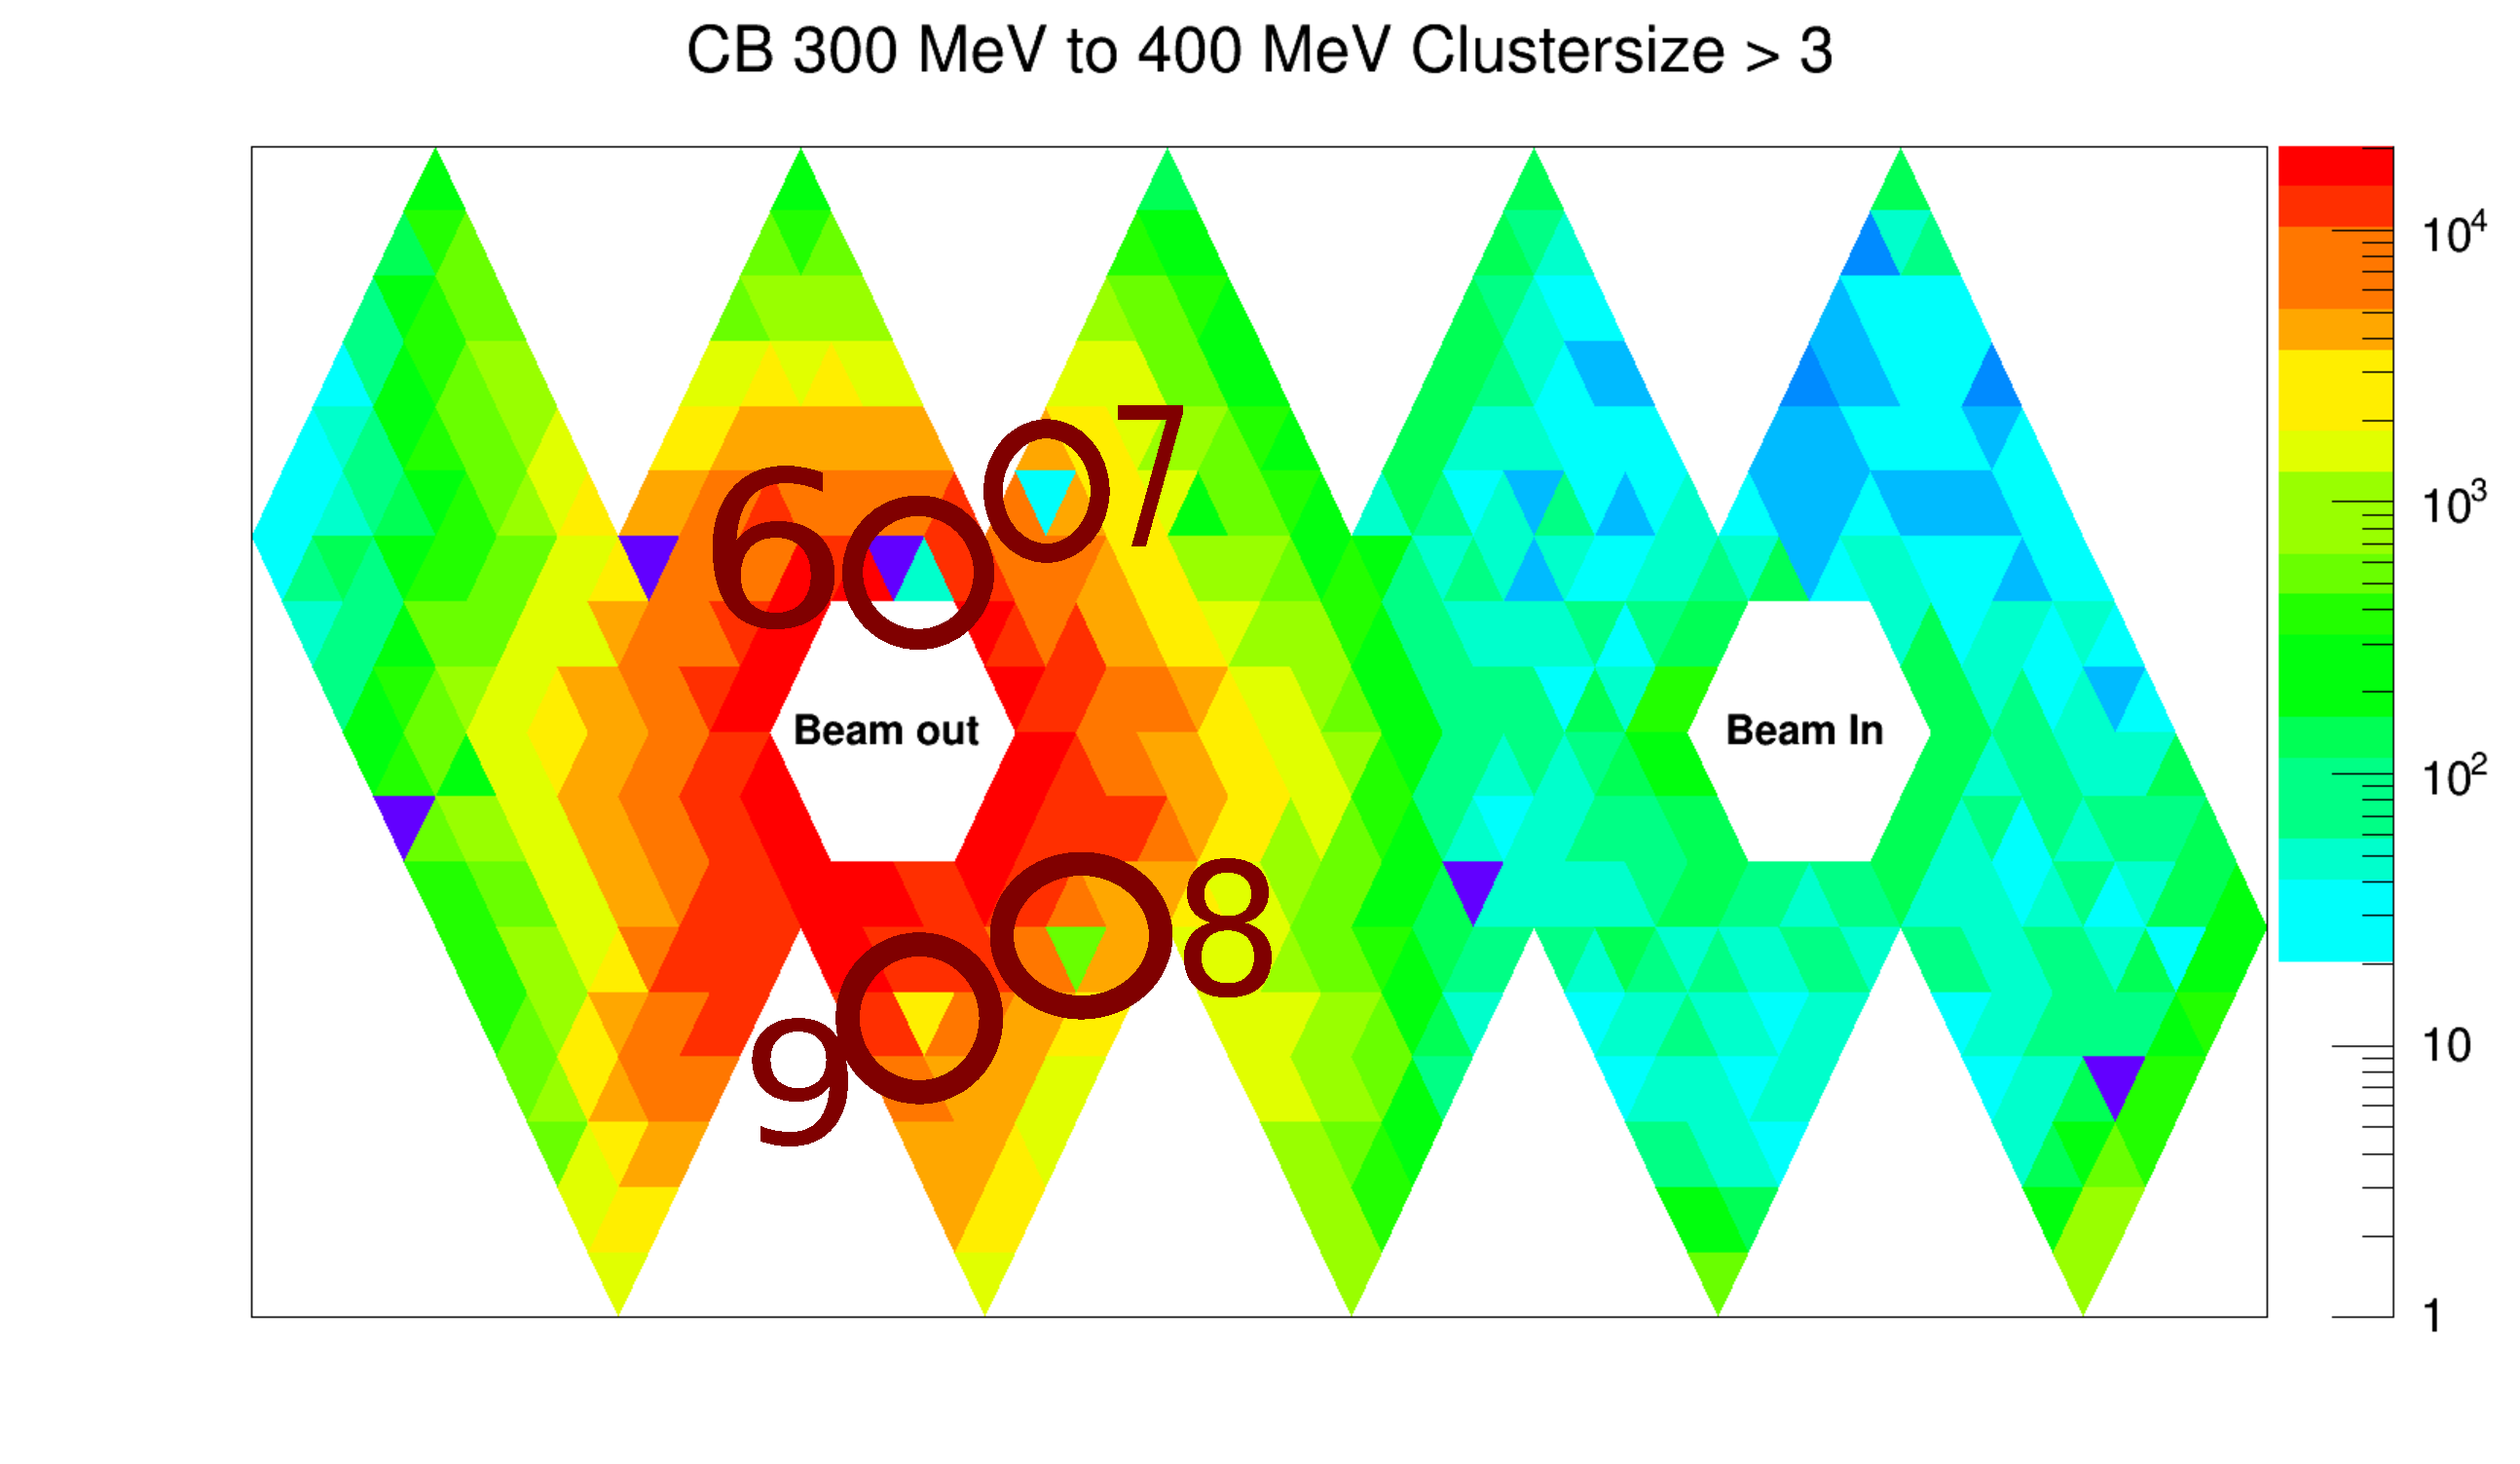
\includegraphics[width=\textwidth]{Pictures/20172504StrahlzeitMoreDead}
			\caption{Beamtime: Marked are probably Dead Crystals}
		\end{minipage}\hfill
		\begin{minipage}[t]{.4\textwidth}
			\centering
			\vspace{0pt}
			\captionof{table}{Beamtime: No. of events for the Dead Crystals and their neighbors}
		\scalebox{0.50}{
			\begin{tabular}{lcc}
				No. in Fig. & Element Number & No. of Hits \\
				
				\hline
				%\rowcolor{LightCyan}
				6& \textcolor{red}{678} &\textcolor{red}{48} \\
				
				& 677&0 \\
				
				& 676& 11808\\ 
				
				
				\hline
				7& \textcolor{red}{17} &\textcolor{red}{21} \\
				
				& 16 & 3311\\
				
				& 18& 7175 \\
				
				& 19& 3439 \\
				
				\hline
				
				8 & \textcolor{red}{125} &\textcolor{red}{513} \\
				
				
				& 122& 6613\\
				
				& 128 & 5307 \\
				
				& 126 & 4103 \\
				
				\hline
				
				9 & \textcolor{red}{89}& \textcolor{red}{2500}\\
				
				& 88& 8591\\
				
				&90&7975 \\
				
				&91&4652 \\
				
				
				
			\end{tabular}
		}	
		\end{minipage}
	\end{figure}
\end{frame}

\begin{frame}
	\frametitle{$\phi$-Distribution in the CB}
	\begin{itemize}
		\item Beamtime October 2014
		\item Photon energy between $200\,\text{MeV}$ and $225\,\text{MeV}$
	\end{itemize}
	\begin{figure}
		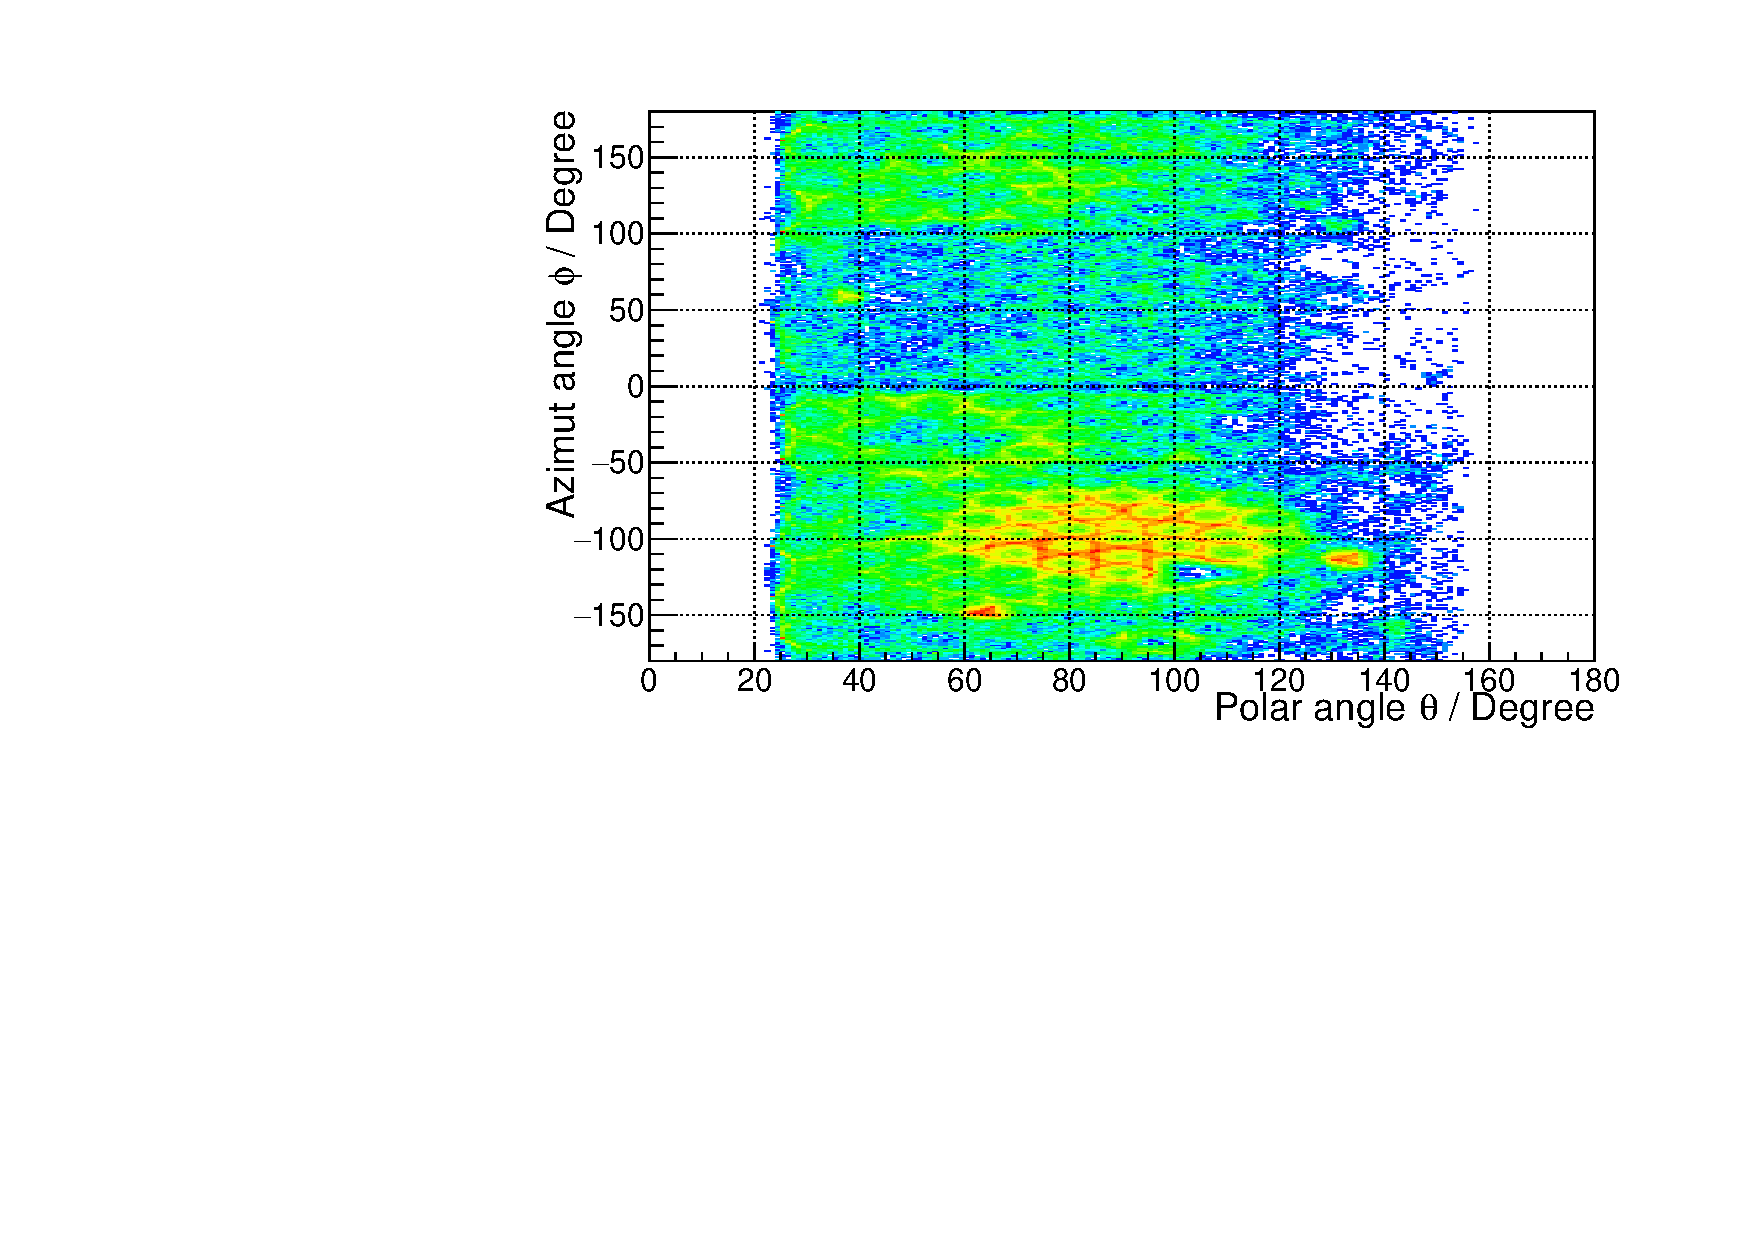
\includegraphics[width=0.75\textwidth]{Pictures/20172404ThetaPhi200MeVBeam}
		\caption{Beamtime: Distribution in the CB}
	\end{figure}
\end{frame}


\section{Conclusion}
\begin{frame}
	\frametitle{Conclusion}
	\begin{itemize}
		\item There is a energy dependency in the detector
		\item The reconstructed opening angle is too big for high energies
		
		$\rightarrow$ wrong reconstruction of the photon impact position is probably the reason for the dependency (Clustering Algorithm) 
		\item The hardware of some PIDs has to be checked (too few or to many events)
		\item There is a strange $\phi$-distribution in the detector
		
		$\rightarrow$ reason for this has also to be determined
	\end{itemize}
\end{frame}
\end{document} 